\documentclass[a4paper,12pt]{article}

% 引入中文支持宏包
\usepackage[UTF8]{ctex}
% 页面边距设置
\usepackage{geometry}
\geometry{left=2.5cm,right=2.5cm,top=2.5cm,bottom=2.5cm}
% 图片与表格
\usepackage{graphicx}
\usepackage{booktabs}
\usepackage{array}
\usepackage{float}
\usepackage{amsmath}
\usepackage{url}
\usepackage{hyperref}

\graphicspath{{ml2_report_assets/}}
\hypersetup{
    colorlinks=true,
    linkcolor=black,
    citecolor=black,
    urlcolor=blue
}

% 设置行间距
\linespread{1.5}

\newcommand{\metric}[1]{\textbf{#1}}
\newcommand{\cls}[1]{\texttt{Class\_#1}}
\newcolumntype{L}[1]{>{\raggedright\arraybackslash}p{#1}}

\begin{document}

\begin{center}
    {\LARGE \textbf{机器学习课程报告：}}\\
    \vspace{0.5em}
    {\LARGE \textbf{少样本细胞图像分类中的尺度校准与病理基础模型迁移}}
\end{center}

\vspace{7.5cm}

\begin{center}
\noindent \textbf{课程名称：} \makebox[5cm]{机器学习} \\
\noindent \textbf{学生姓名：} \underline{\makebox[5cm]{公开版略}} \\
\noindent \textbf{学生学号：} \underline{\makebox[5cm]{公开版略}} \\
\noindent \textbf{授课教师：} \makebox[5cm]{公开版略} \\
\noindent \textbf{日期：} 2026年 7 月 4 日
\end{center}

\newpage

\section{实验背景与数据探索}

\subsection{任务定义与问题拆解}

本次期末任务要求在每类仅 50 张训练样本的条件下构建 5 分类图像分类器，并在大规模、类别不均衡的测试集上提交预测结果。训练集共 250 张 \(32\times32\) RGB 图像，类别为 \texttt{Class\_0} 到 \texttt{Class\_4}；测试集共 61,881 张无标签图像。评价指标采用 macro-F1 与 balanced accuracy，因此模型不能只优化总体准确率，而要让每个类别都形成可用的召回和精度边界。

这个问题可以拆成一个大问题和三个小问题。大问题是：如何在极少有标签样本下迁移一个足够强的视觉表示，并使它泛化到大规模不均衡测试集。小问题分别是：第一，\(32\times32\) 单细胞图像与 \(224\times224\) 病理基础模型输入视野之间存在尺度错配；第二，250 张样本不足以支持全量微调，需要参数高效微调；第三，测试集没有标签但规模很大，若使用伪标签，必须避免伪标签被容易类别主导。换言之，本项目的 research gap 不是“再训练一个普通 5 分类 CNN”，而是如何把在大尺寸病理 tile 上预训练的基础模型，可靠地迁移到低分辨率、中心细胞级别、标签极少的分类任务上。

内部模型选择使用如下 selection score：
\begin{equation}
    \mathrm{selection}
    = \frac{1}{2}\mathrm{macro\text{-}F1}
    + \frac{1}{2}\mathrm{balanced\ accuracy}.
\end{equation}
其中 macro-F1 对每个类别的 F1 取平均，balanced accuracy 对每个类别的 recall 取平均。二者都削弱了测试集类别不均衡对评价的影响，也使弱类错误更容易反映到总分中。

\subsection{数据集统计分析}

图 \ref{fig:dataset-counts} 展示训练集的类别分布。训练集在标签数量上完全均衡，每类 50 张，但样本量极小；测试集则有 61,881 张无标签图像，规模约为训练集的 247.5 倍。这个比例说明测试集不仅是最终评价集合，也提供了大量无标签分布信息；但由于测试标签不可见，任何利用测试集的策略都只能基于 teacher prediction、confidence 或 soft label，不能引入隐藏标签。

\begin{figure}[H]
    \centering
    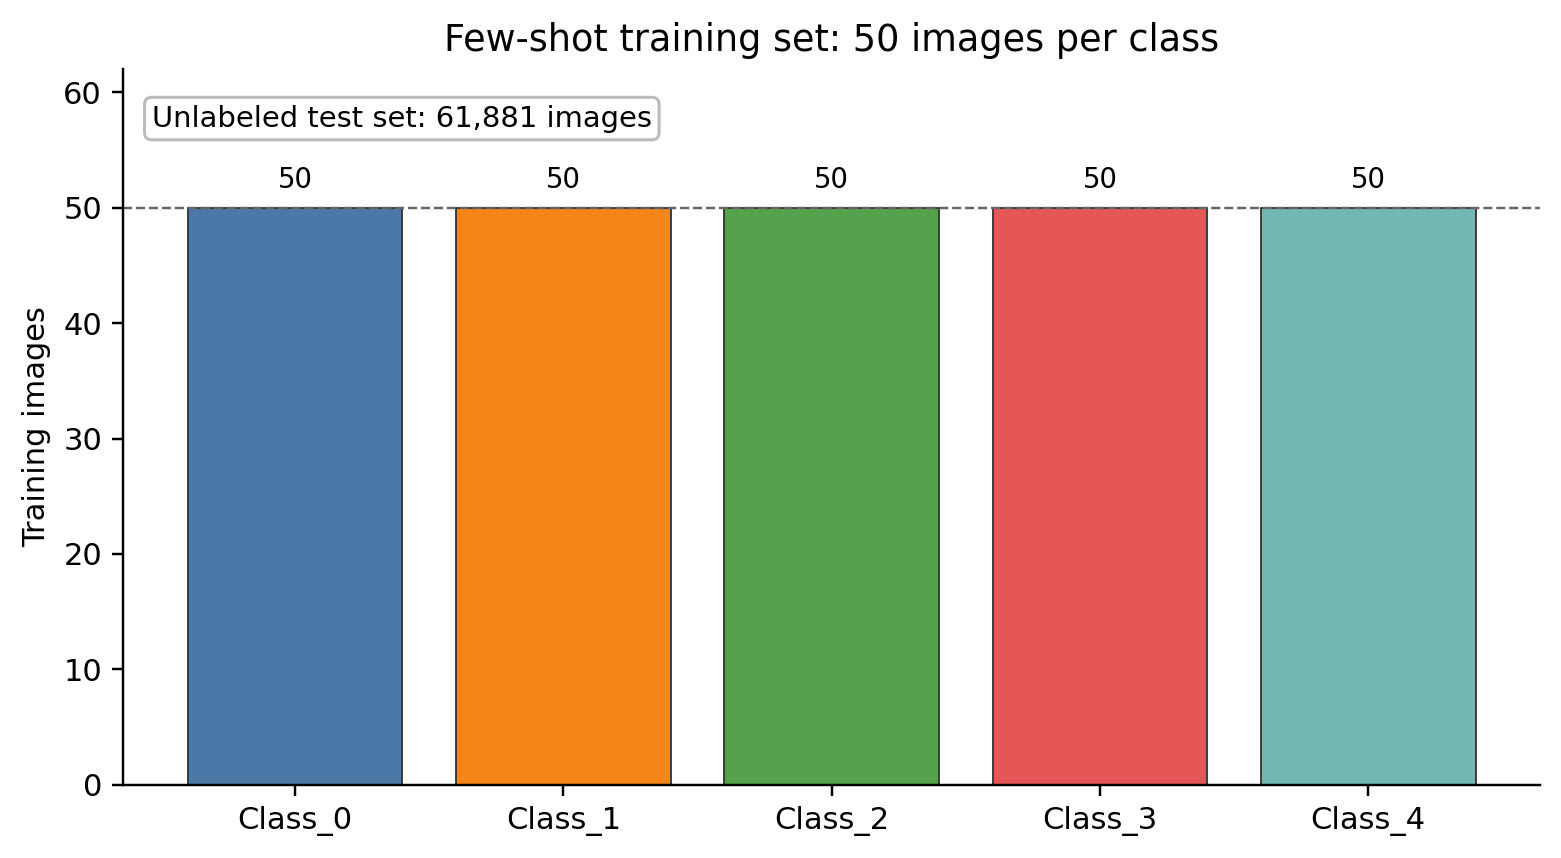
\includegraphics[width=0.82\textwidth]{dataset_counts.png}
    \caption{训练集每类 50 张，测试集为 61,881 张无标签图像。该分布决定了模型选择应优先关注 macro-F1 与 balanced accuracy。}
    \label{fig:dataset-counts}
\end{figure}

图 \ref{fig:contact-sheet} 展示不同类别的放大样本。每张原图只有 \(32\times32\) 像素，放大后可以看到两个特点：第一，类别差异主要来自细胞核形态、染色深浅、胞质边界和局部纹理，而不是大尺度物体轮廓；第二，同一类别内部也存在明显颜色和形态变化。例如 \(\cls{3}\) 的训练图平均亮度最高，\(\cls{4}\) 的平均局部对比度最高（见表 \ref{tab:train-image-stats}），说明模型如果只记忆颜色强弱，很容易把类别内变化误当作类别边界。因此，后续方法需要依赖病理基础模型的形态先验，而不能只做浅层颜色阈值或手工特征分类。

\begin{figure}[H]
    \centering
    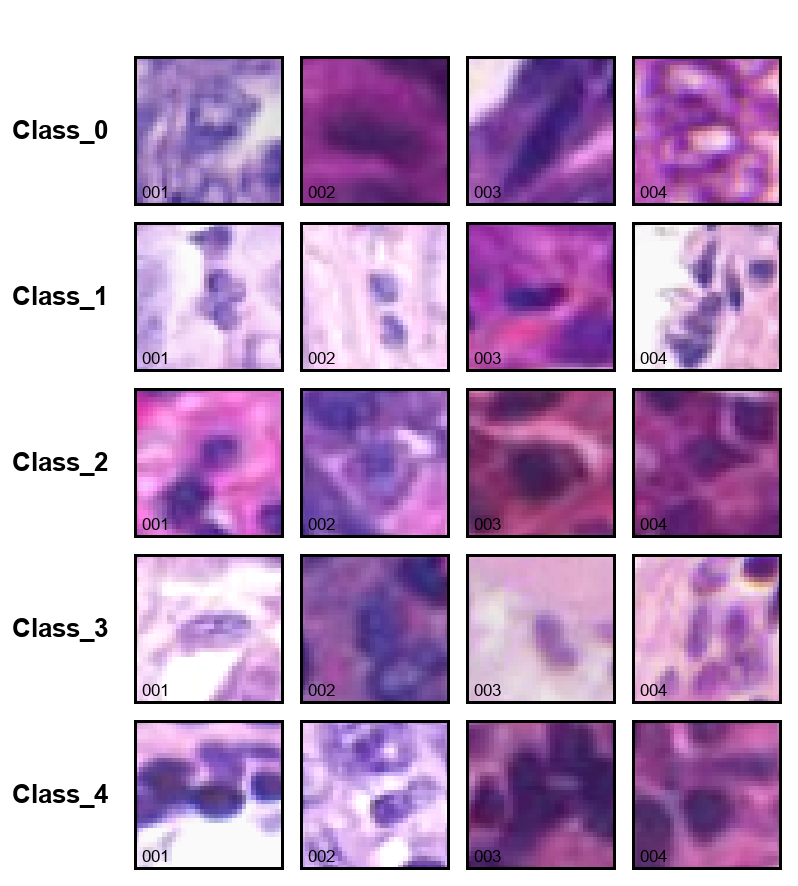
\includegraphics[width=0.88\textwidth]{class_examples_large.png}
    \caption{训练样本放大示例。每行对应一个类别，每个小图由 \(32\times32\) 原图最近邻放大得到，便于观察低分辨率下的核形态和染色纹理差异。}
    \label{fig:contact-sheet}
\end{figure}

\begin{table}[H]
    \centering
    \caption{训练集按类别统计的图像均值与局部对比度}
    \label{tab:train-image-stats}
    \small
    \begin{tabular}{lrrr}
        \toprule
        \textbf{类别} & \textbf{样本数} & \textbf{平均像素均值} & \textbf{平均局部对比度} \\
        \midrule
        \cls{0} & 50 & 0.5914 & 0.1585 \\
        \cls{1} & 50 & 0.6127 & 0.1699 \\
        \cls{2} & 50 & 0.6080 & 0.1835 \\
        \cls{3} & 50 & 0.6745 & 0.1574 \\
        \cls{4} & 50 & 0.6188 & 0.1922 \\
        \bottomrule
    \end{tabular}
\end{table}

进一步的内容偏移分析如图 \ref{fig:content-shift} 所示。测试集的平均图像亮度为 0.6309，高于训练集的 0.6181，差值约为 \(+2.1\%\)；测试集平均对比度为 0.1125，低于训练集的 0.1253，差值约为 \(-10.2\%\)。误差线表示 p10--p90 区间，可以看到训练集与测试集仍有大量重叠，因此这里不能夸大为剧烈分布漂移。更合理的解释是：测试集整体略亮、对比度略低，并且覆盖的样本数量远大于训练集。这个证据支持两点设计选择：一是使用轻微 brightness/contrast/saturation jitter 来提高颜色鲁棒性；二是利用伪标签自训练感知测试集分布，但必须用低权重 soft label 控制 teacher noise。

\begin{figure}[H]
    \centering
    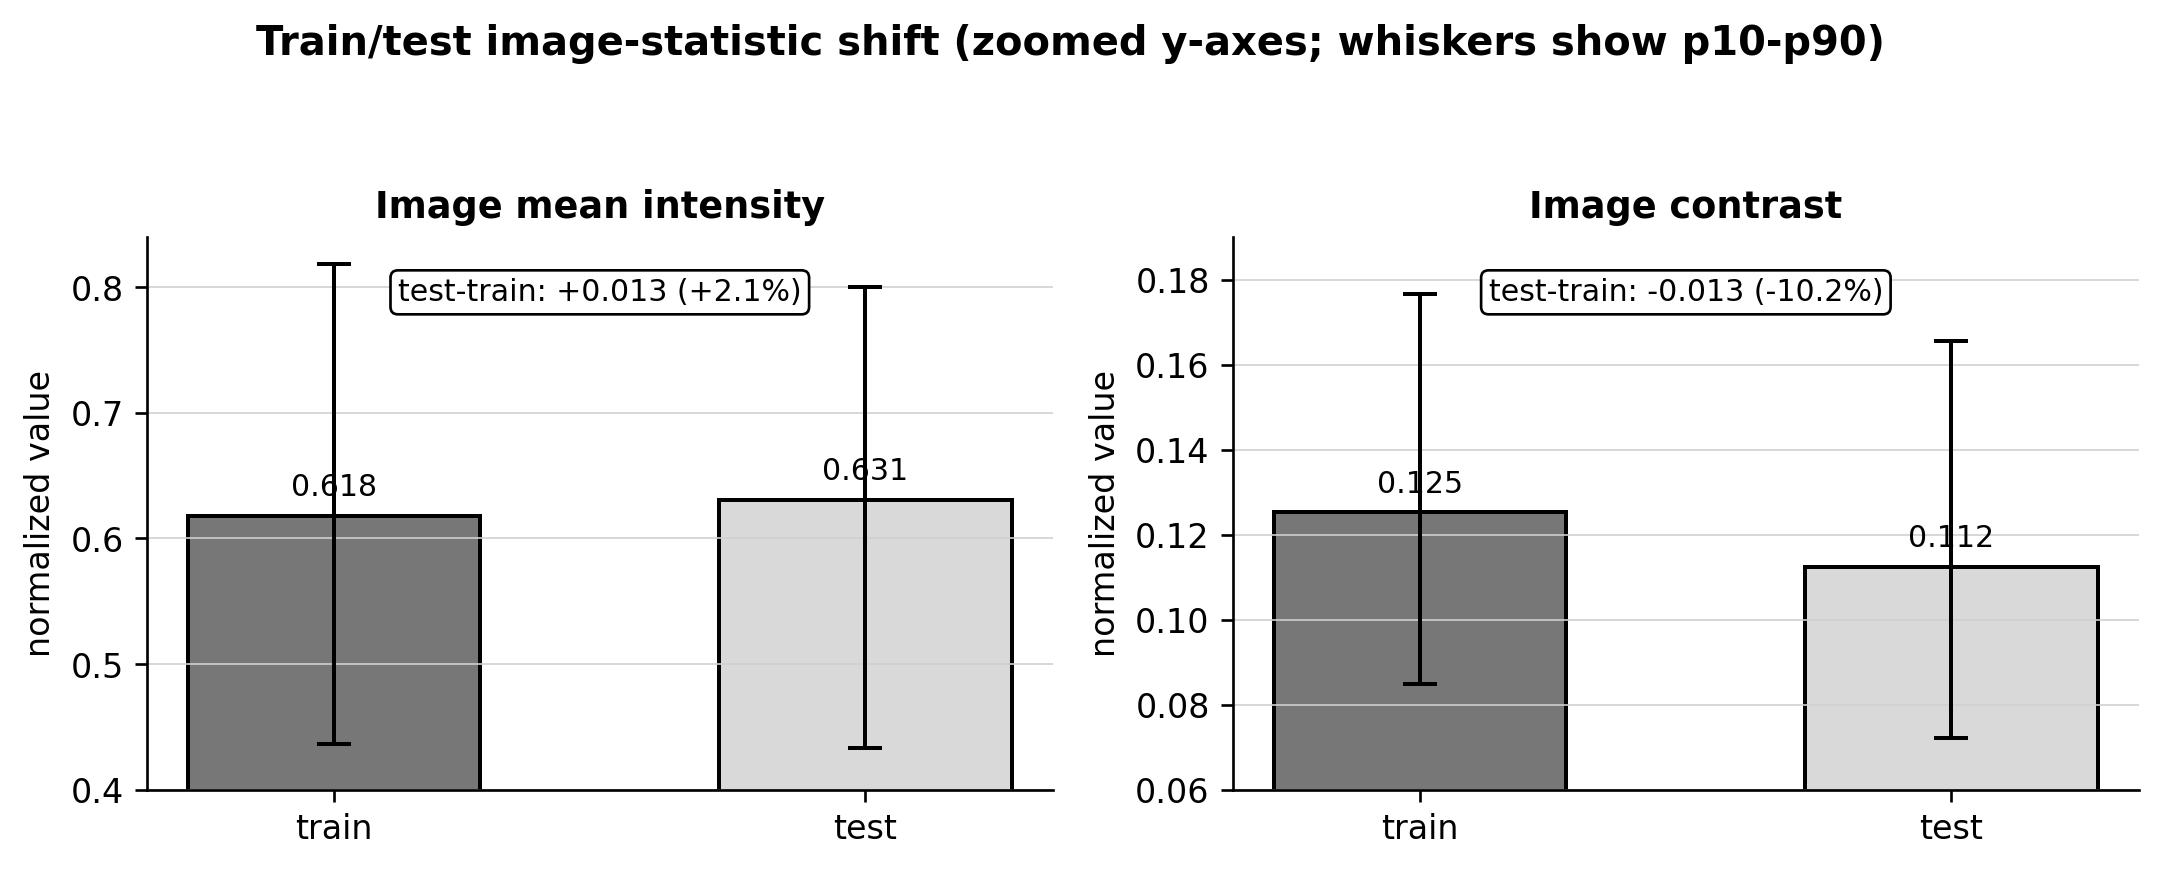
\includegraphics[width=\textwidth]{train_test_content_shift_zoomed.png}
    \caption{训练集与测试集图像统计差异。纵轴采用局部范围以显示轻度均值差异，误差线表示 p10--p90 区间；该图说明颜色/对比度存在轻度 shift，但分布仍明显重叠。}
    \label{fig:content-shift}
\end{figure}

\subsection{数据预处理与数据增强}

项目探索中最关键的发现是输入尺度校准。UNI2-h 等病理基础模型通常以 \(224\times224\) 病理图像块为输入，ViT 主干会将图像划分为固定 patch token 进行建模 \cite{dosovitskiy2021vit}。如果把 \(32\times32\) 单细胞图像直接拉伸到 \(224\times224\)，每条边会被放大 7 倍，细胞会占满整张画布。此时模型看到的是一个被过度放大的细胞结构，而不是一个位于病理视野中的局部目标；插值还会放大低分辨率纹理伪影，使 ViT token 捕获到的局部频率和预训练时的病理 tile 不一致。

最终方法采用 \texttt{CenterScalePad}：先将 \(32\times32\) 图像缩放到 \(64\times64\)，再以白色背景居中填充到 \(224\times224\)。如图 \ref{fig:scale-preprocess} 所示，这种处理保留了单细胞作为中心局部目标的语义，也减少了 \(32\rightarrow224\) 直接插值带来的纹理伪影。课堂汇报中总结的核心结论正是：先让基础模型看到合理尺度的细胞，再讨论微调与伪标签，收益比盲目堆叠 backbone 更稳定。

\begin{figure}[H]
    \centering
    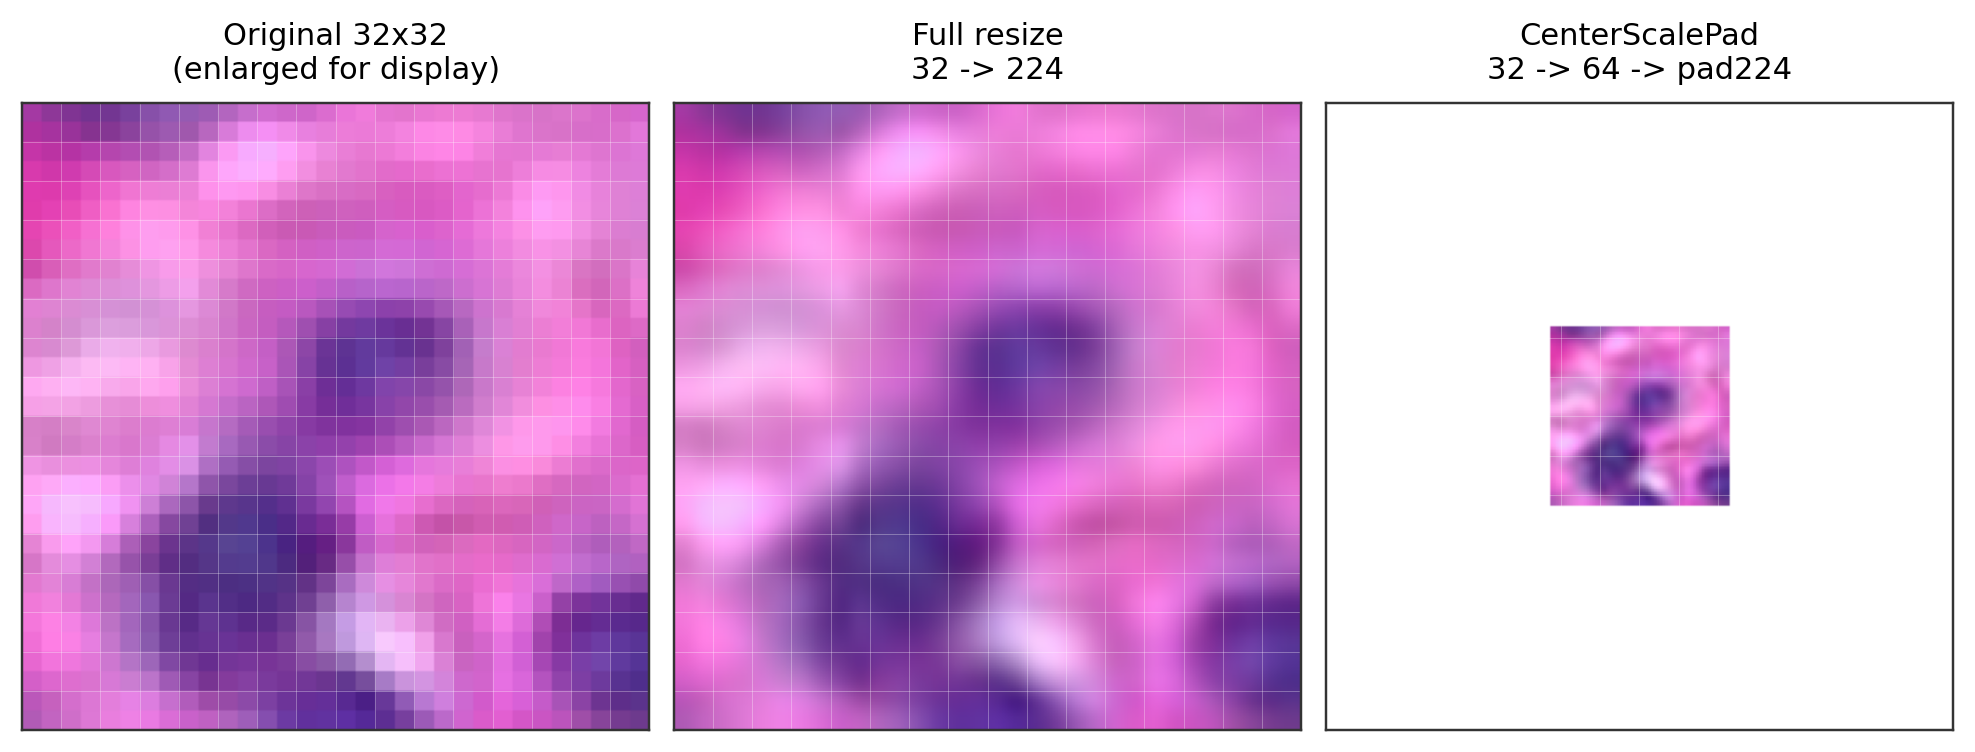
\includegraphics[width=\textwidth]{scale_preprocess_comparison.png}
    \caption{输入尺度校准示意。直接 full resize 会让单细胞占满 \(224\times224\) 画布，而 CenterScalePad 将细胞保留为中心局部目标。浅色网格表示 UNI2-h 的 ViT token 划分。}
    \label{fig:scale-preprocess}
\end{figure}

训练阶段只使用温和增强，包括水平翻转、垂直翻转、90 度旋转、小幅平移以及轻微亮度、对比度和饱和度扰动。这个选择与前面的数据观察一致：图像方向通常不是细胞类别本身，轻度翻转和旋转可以扩展形态方向；测试集亮度略高、对比度略低，轻微颜色扰动可以提高染色鲁棒性。但没有使用强随机裁剪、强 CutMix 或强 MixUp，因为 \(32\times32\) 图像过小，强空间增强可能直接切掉细胞核或制造不存在的混合细胞形态，从而把增强变成标签噪声。

\section{模型架构与设计}

\subsection{模型选型}

最终方案采用 UNI2-h 作为主干。UNI 系列是面向 H\&E 病理图像的大规模自监督基础模型 \cite{chen2024uni}，UNI2-h 权重来自 Hugging Face 的 \texttt{MahmoodLab/UNI2-h} 模型仓库，其模型卡说明该模型和相关代码以 CC-BY-NC-ND-4.0 许可证发布，仅限非商业学术研究使用 \cite{mahmoodlab2026uni2h}。选择 UNI2-h 的原因有三点：第一，任务图像来自病理/细胞形态域，病理基础模型比普通自然图像模型更有先验；第二，250 张训练图不足以从头学习稳定表征；第三，后续消融显示修正输入尺度后的单 UNI2-h 已超过早期多 backbone fusion。

整体架构如图 \ref{fig:architecture} 所示。原始 \(32\times32\) RGB 图像首先经过 \texttt{CenterScalePad}（参数 \texttt{scale\_to=64}）：图像被缩放到 \(64\times64\)，再居中粘贴到白色 \(224\times224\) 画布上。处理后的图像输入 UNI2-h ViT-H/14 主干，得到 1536 维视觉表征；主干的预训练参数保持冻结，仅在 self-attention 的 \texttt{qkv} 与 \texttt{proj} 线性层加入 rsLoRA 低秩更新，并训练一个 5 类线性分类头。最终提交阶段只使用一个 full-250 single-refit 模型，不做模型集成，也不进行测试时增强。

\begin{figure}[H]
    \centering
    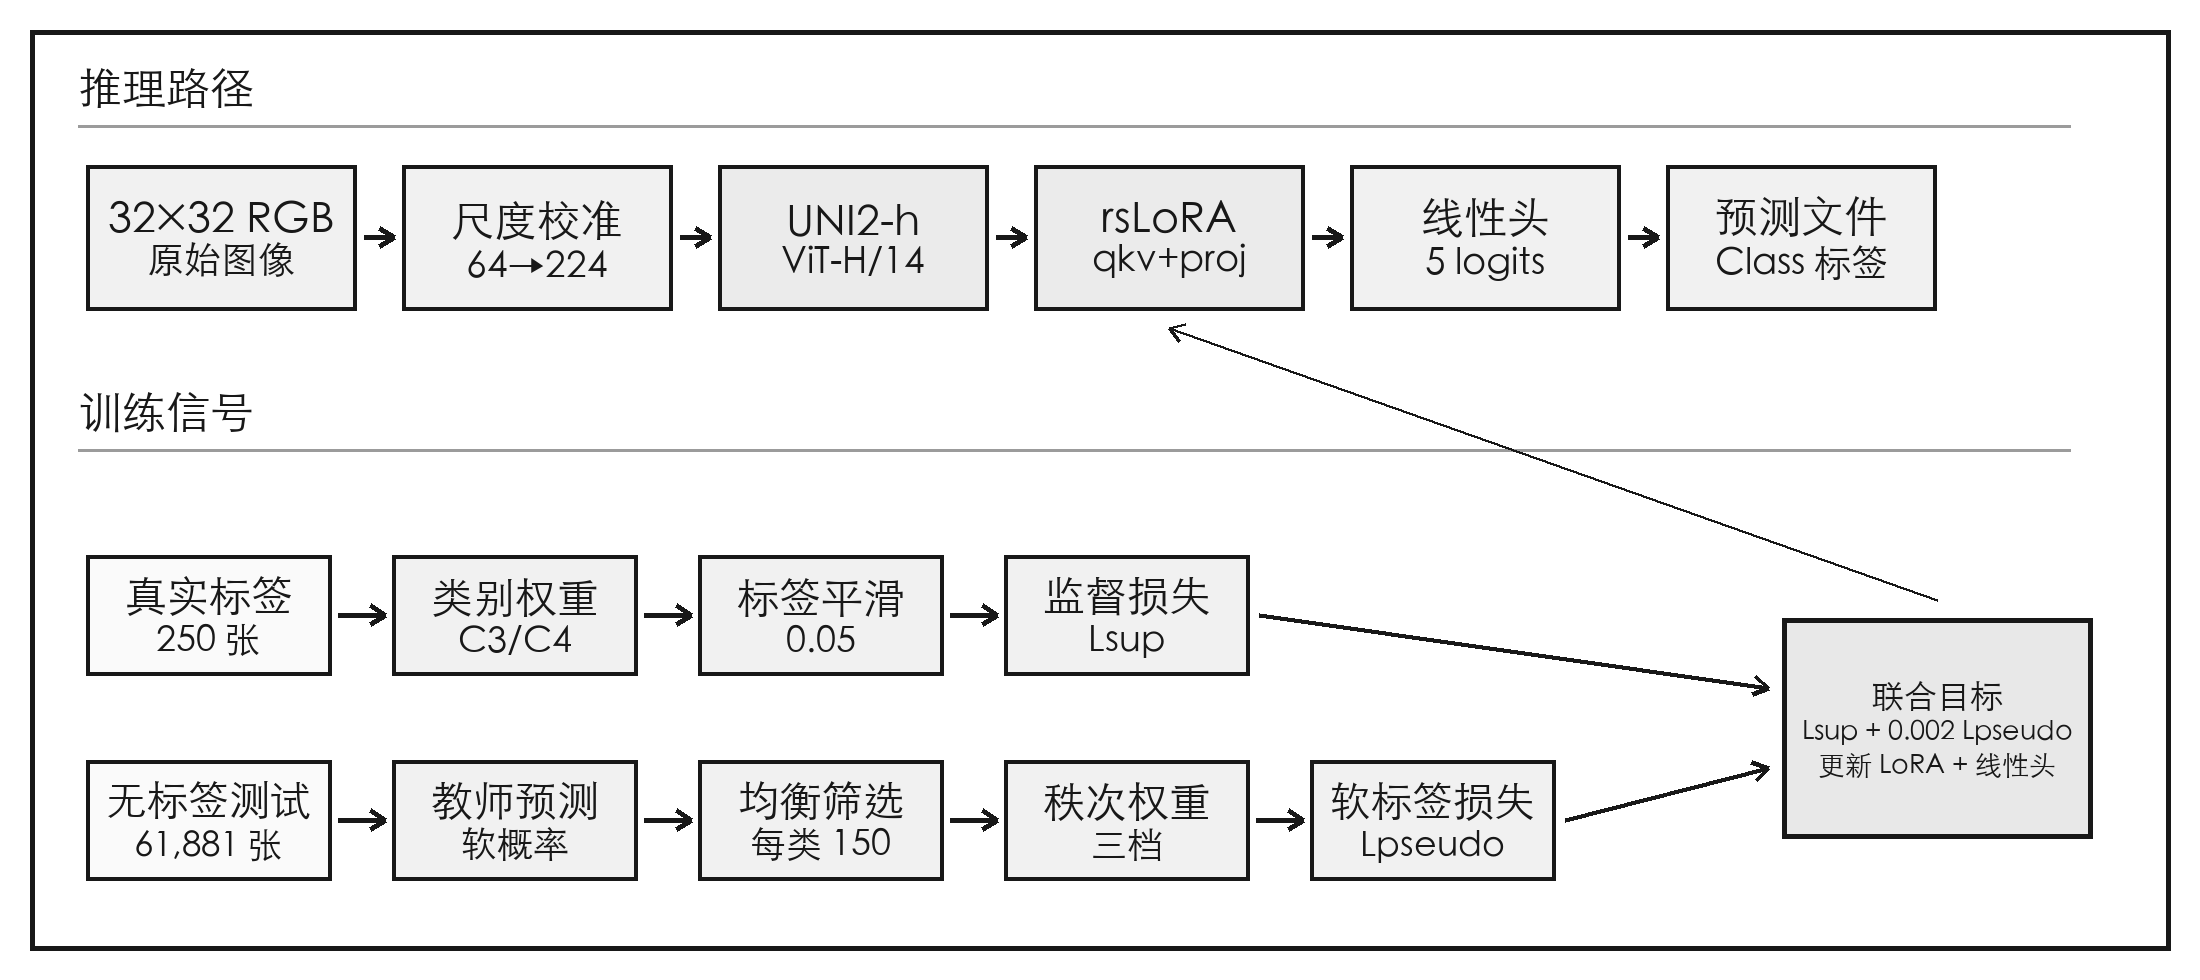
\includegraphics[width=\textwidth]{architecture_pipeline.png}
    \caption{最终模型的推理路径与训练信号示意。上方为单模型预测流程，下方为真实标签监督损失与均衡软伪标签损失共同优化 LoRA 参数和分类头的训练路径。}
    \label{fig:architecture}
\end{figure}

\subsection{训练策略配置}

最终微调方式是 rsLoRA。LoRA 的基本思想是在冻结预训练权重的同时，为线性层增加低秩可训练更新，从而显著减少下游任务所需训练参数 \cite{hu2022lora}。本项目只对 attention \texttt{qkv+proj} 注入 LoRA，配置为 \(r=16\)、\(\alpha=32\)、dropout 0.05、\texttt{bias=none}，并保存分类头。参数审计显示，最终模型总参数量为 684,948,490，可训练参数为 3,554,314，可训练比例约 0.52\%。这种设计比只训练线性头有更强适配能力，又比全量微调更适合 250 张样本的小数据场景。

主要训练配置见表 \ref{tab:final-config}。训练使用 bf16 精度、batch size 16、weight decay 0.01、label smoothing 0.05、最大梯度范数 1.0，并启用 gradient checkpointing。类别权重为 \(\cls{3}=1.25\)、\(\cls{4}=1.10\)，其余类别为 1.00，用于提高难类在损失函数中的梯度权重。

\begin{table}[H]
    \centering
    \caption[Final model configuration]{最终模型与训练配置}
    \label{tab:final-config}
    \small
        \begin{tabular}{l>{\raggedright\arraybackslash}p{9.5cm}}
        \toprule
        \textbf{项目} & \textbf{配置} \\
        \midrule
        主干模型 & UNI2-h, ViT-H/14, feature dimension 1536, input size 224 \\
        输入处理 & \(32\times32 \rightarrow 64\times64 \rightarrow 224\times224\) CenterScalePad，白色填充 RGB \([255,255,255]\) \\
        可训练模块 & attention \texttt{qkv+proj} 的 rsLoRA 参数与 5 类线性分类头 \\
        LoRA 配置 & \(r=16\), \(\alpha=32\), dropout 0.05, \texttt{bias=none}, \texttt{use\_rslora=true} \\
        优化与正则 & bf16, batch size 16, weight decay 0.01, label smoothing 0.05, max grad norm 1.0, gradient checkpointing \\
        类别权重 & \(\cls{0}=1.00\), \(\cls{1}=1.00\), \(\cls{2}=1.00\), \(\cls{3}=1.25\), \(\cls{4}=1.10\) \\
        损失函数 & 真实样本使用类别加权 hard cross entropy；伪标签样本使用带样本权重的 soft-label cross entropy，\(\lambda_{\mathrm{pseudo}}=0.002\) \\
        伪标签 & 750 张，5 类各 150 张，rank 1--50/51--100/101--150 的权重倍率为 1.00/0.25/0.10 \\
        最终提交 & full-250 single-refit，训练 11 epoch，单模型预测，无模型集成与测试时增强 \\
        \bottomrule
    \end{tabular}
\end{table}

\subsection{最终选用方法详细阐述}

最终方法可以表述为一个两阶段的参数高效半监督迁移流程。第一阶段在 5-fold OOF 上比较尺度、微调方式、类别权重和伪标签策略；第二阶段固定 OOF 选出的配置，在 250 张有标签样本和筛选后的软伪标签上训练一个 single-refit 模型并生成提交文件。该流程的核心不是增加模型数量，而是使输入尺度、可训练参数规模和无标签信息利用方式同时保持受控。

输入变换记为 \(T_{\mathrm{scale64}}\)。对每张原图 \(x\)，先将 \(32\times32\) 图像按双线性插值缩放到 \(64\times64\)，再放置到 \(224\times224\) 白色画布中心。与直接 full resize 相比，这个变换保留了细胞作为局部目标的相对尺度，使 UNI2-h 的 ViT token 网格看到的目标大小更接近病理 tile 预训练中的局部组织结构。尺度消融结果表明，full224 明显弱于 scale48 和 scale64，因此尺度校准被保留为最终架构的第一步。

监督训练目标由真实标签损失和软伪标签损失组成：
\begin{equation}
    \mathcal{L}
    =
    \mathcal{L}_{\mathrm{sup}}
    +
    \lambda_{\mathrm{pseudo}}\mathcal{L}_{\mathrm{pseudo}},
    \quad
    \lambda_{\mathrm{pseudo}}=0.002.
\end{equation}
其中 \(\mathcal{L}_{\mathrm{sup}}\) 是带标签平滑的类别加权 hard CE。类别权重中，\(\cls{3}\) 为 1.25，\(\cls{4}\) 为 1.10，用于提高难类样本在梯度更新中的影响。伪标签项 \(\mathcal{L}_{\mathrm{pseudo}}\) 使用教师模型输出的 5 维概率分布作为 soft target，而不是把最高概率类别硬化为 one-hot 标签，从而保留教师模型对相近类别不确定性的表达。

均衡软伪标签的筛选方式如下。首先使用已验证的 UNI2-h scale64 教师模型对 61,881 张测试图像产生类别概率；随后在每个预测类别内部按置信度排序，并分别选取前 150 张，得到 750 张伪标签样本。为降低低置信伪标签的影响，每类 rank 1--50、51--100、101--150 的样本权重倍率分别为 1.00、0.25、0.10。训练记录显示，虽然伪标签样本数量是有标签样本的 3 倍，但伪标签有效权重和为 0.2357；因此该项在优化中主要提供低强度的测试分布约束，而不会替代真实标签监督。

最终 full-refit 的训练轮数由交叉验证阶段的最优轮次分布确定。五折中以 macro-F1 选择的最佳轮次为 \([8,24,14,11,11]\)，其中位数为 11；因此最终模型在相同训练配方下训练 11 个 epoch。该规则将 full-refit 的训练时长约束在交叉验证观察到的有效区间内，降低在全训练集上过度延长训练的风险。

\section{实验结果与可视化}

\subsection{训练稳定性与评价口径}

本节从三个层次报告最终方案的实验结果。首先，训练曲线用于检查 full-refit 阶段的优化过程是否稳定；其次，5-fold OOF 指标用于评估在有标签训练集上的模型选择质量；最后，测试集预测分布与错误案例用于分析无标签大规模测试分布上的潜在风险。三类证据的含义不同：OOF 分数是可比较的本地验证结果，测试集预测分布只是无标签诊断，不能被解释为隐藏测试集性能。

图 \ref{fig:loss} 展示最终 single-refit 模型的训练损失。该阶段使用 250 张真实标签图像和 750 张均衡软伪标签图像，batch 中伪标签样本比例为 0.75；但由于伪标签损失被 \(\lambda_{\mathrm{pseudo}}=0.002\) 缩放，且伪标签有效权重和仅为 0.2357，优化过程仍以真实标签监督为主。损失从第 1 个 epoch 的 2.6464 降至第 4 个 epoch 的 0.6714，随后进入缓慢下降区间；第 8 个 epoch 为 0.4379，第 11 个 epoch 为 0.4297。该趋势说明 LoRA 参数和分类头能够被稳定优化，没有出现损失发散或训练中断。但由于 full-refit 阶段没有独立验证集，这条曲线只用于训练稳定性检查，不作为泛化能力的直接证据。

\begin{figure}[H]
    \centering
    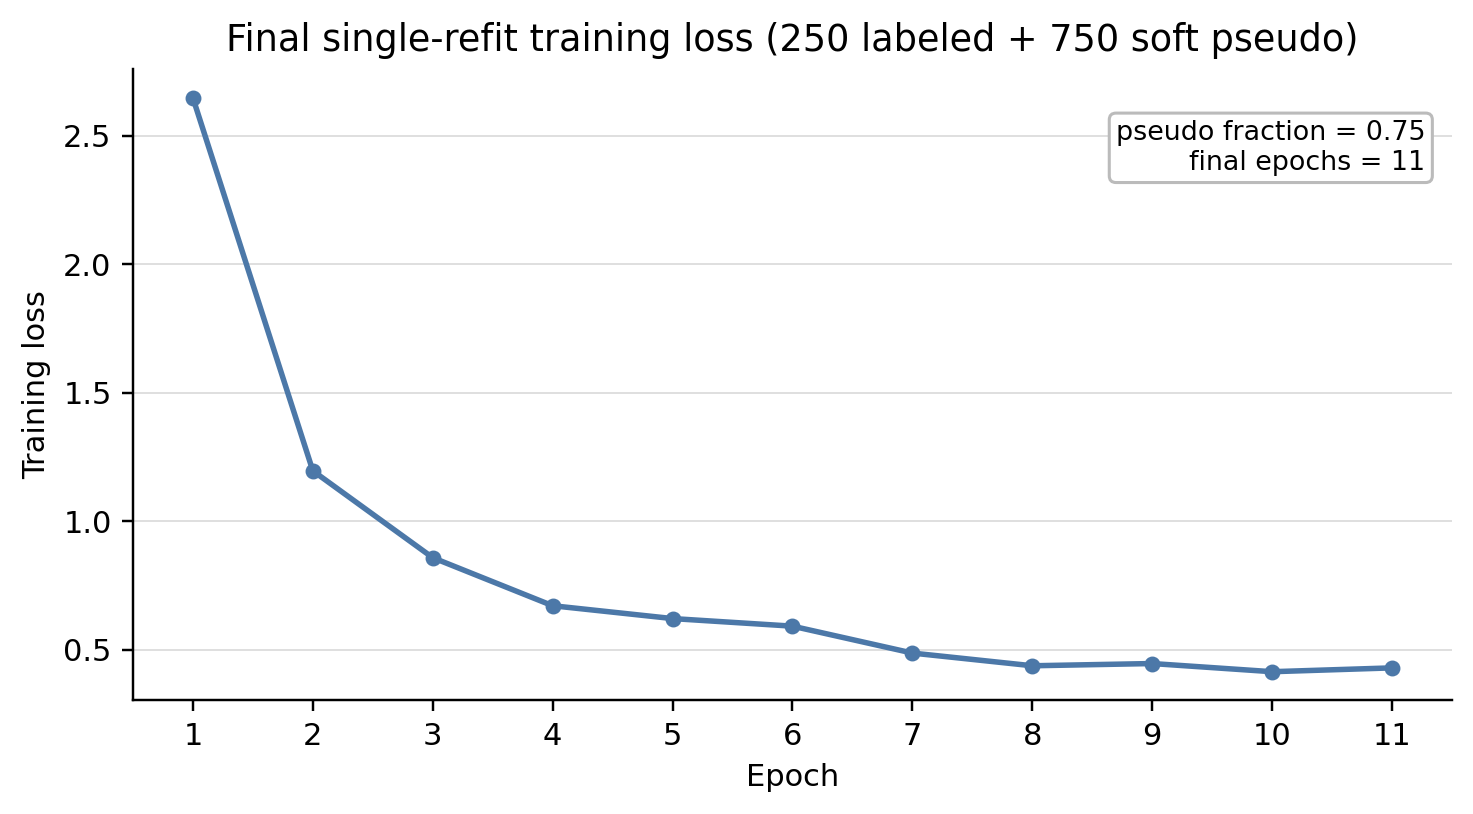
\includegraphics[width=0.82\textwidth]{final_single_refit_loss.png}
    \caption{最终 single-refit 训练损失。训练数据由 250 张真实标签图像与 750 张软伪标签图像组成，最终训练 11 epoch。}
    \label{fig:loss}
\end{figure}

\subsection{OOF 分类结果}

最终模型的本地 5-fold OOF 结果如表 \ref{tab:oof-classification} 所示。OOF 评估中，每张训练图像只由未见过该样本的折外模型预测，因此比直接在训练集上评估更能反映少样本设置下的模型选择质量。最终 macro-F1 为 0.8662，balanced accuracy 为 0.8680，selection score 为 0.8671。由于训练集每类均为 50 张，balanced accuracy 与总体 accuracy 在该 OOF 汇总上数值相同；但在课程隐藏测试集类别不均衡的设定下，balanced accuracy 仍是更合适的类别均衡评价指标。

\begin{table}[H]
    \centering
    \caption{最终 UNI2-h scale64 soft150 lam002 的 5-fold OOF 分类指标}
    \label{tab:oof-classification}
    \small
    \begin{tabular}{lrrrr}
        \toprule
        \textbf{类别} & \textbf{Precision} & \textbf{Recall} & \textbf{F1-score} & \textbf{Support} \\
        \midrule
        \cls{0} & 0.9231 & 0.9600 & 0.9412 & 50 \\
        \cls{1} & 0.9245 & 0.9800 & 0.9515 & 50 \\
        \cls{2} & 0.8302 & 0.8800 & 0.8544 & 50 \\
        \cls{3} & 0.8636 & 0.7600 & 0.8085 & 50 \\
        \cls{4} & 0.7917 & 0.7600 & 0.7755 & 50 \\
        \midrule
        \textbf{Macro average} & 0.8666 & 0.8680 & 0.8662 & 250 \\
        \bottomrule
    \end{tabular}
\end{table}

从类别维度看，模型在 \(\cls{0}\) 和 \(\cls{1}\) 上表现最稳定，recall 分别为 0.9600 和 0.9800，F1-score 分别为 0.9412 和 0.9515。这说明尺度校准后的 UNI2-h 表征可以较好地区分一部分形态边界清晰的类别。相对地，\(\cls{3}\) 和 \(\cls{4}\) 的 recall 均为 0.7600，F1-score 分别为 0.8085 和 0.7755，是最终模型的主要薄弱环节。由于每折每类验证样本只有约 10 张，这些数值不应被理解为稳定的总体估计，而应被视为类别间难度差异和错误方向的证据。

混淆矩阵进一步揭示了弱类错误的结构。最终 OOF 共 33 个错误样本，其中真实类别属于 \(\cls{2}\)、\(\cls{3}\)、\(\cls{4}\) 的错误为 30 个，占全部错误的 90.9\%。具体而言，\(\cls{3}\) 有 12 个样本被错分，其中 6 个被预测为 \(\cls{4}\)；\(\cls{4}\) 也有 12 个样本被错分，其中 5 个被预测为 \(\cls{2}\)，4 个被预测为 \(\cls{3}\)。这说明最终模型的主要困难不是所有类别均匀退化，而是集中在形态相近的中后段类别之间。难类加权和均衡伪标签因此具有明确动机：前者提高弱类在监督损失中的梯度权重，后者避免无标签扩展过程只服务于容易类别。

\begin{figure}[H]
    \centering
    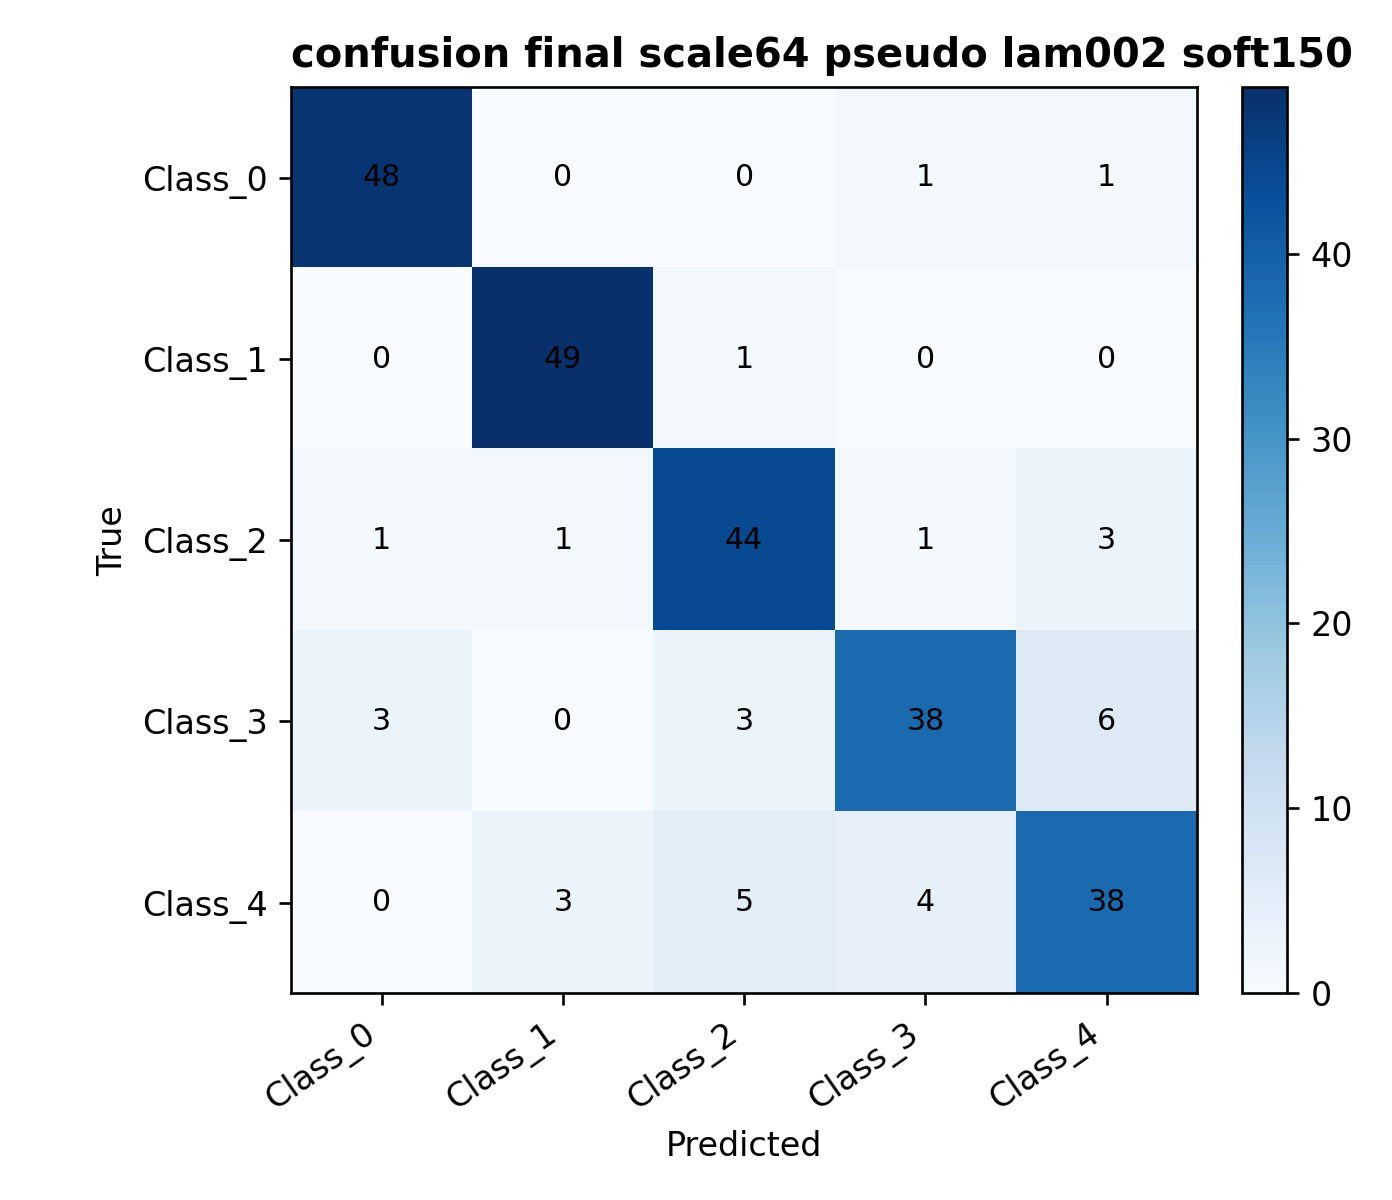
\includegraphics[width=0.78\textwidth]{confusion_final_scale64_pseudo_lam002_soft150.png}
    \caption{最终模型的 5-fold OOF 混淆矩阵。主要误差集中在 \(\cls{2}\)、\(\cls{3}\)、\(\cls{4}\) 之间。}
    \label{fig:confusion}
\end{figure}

\begin{figure}[H]
    \centering
    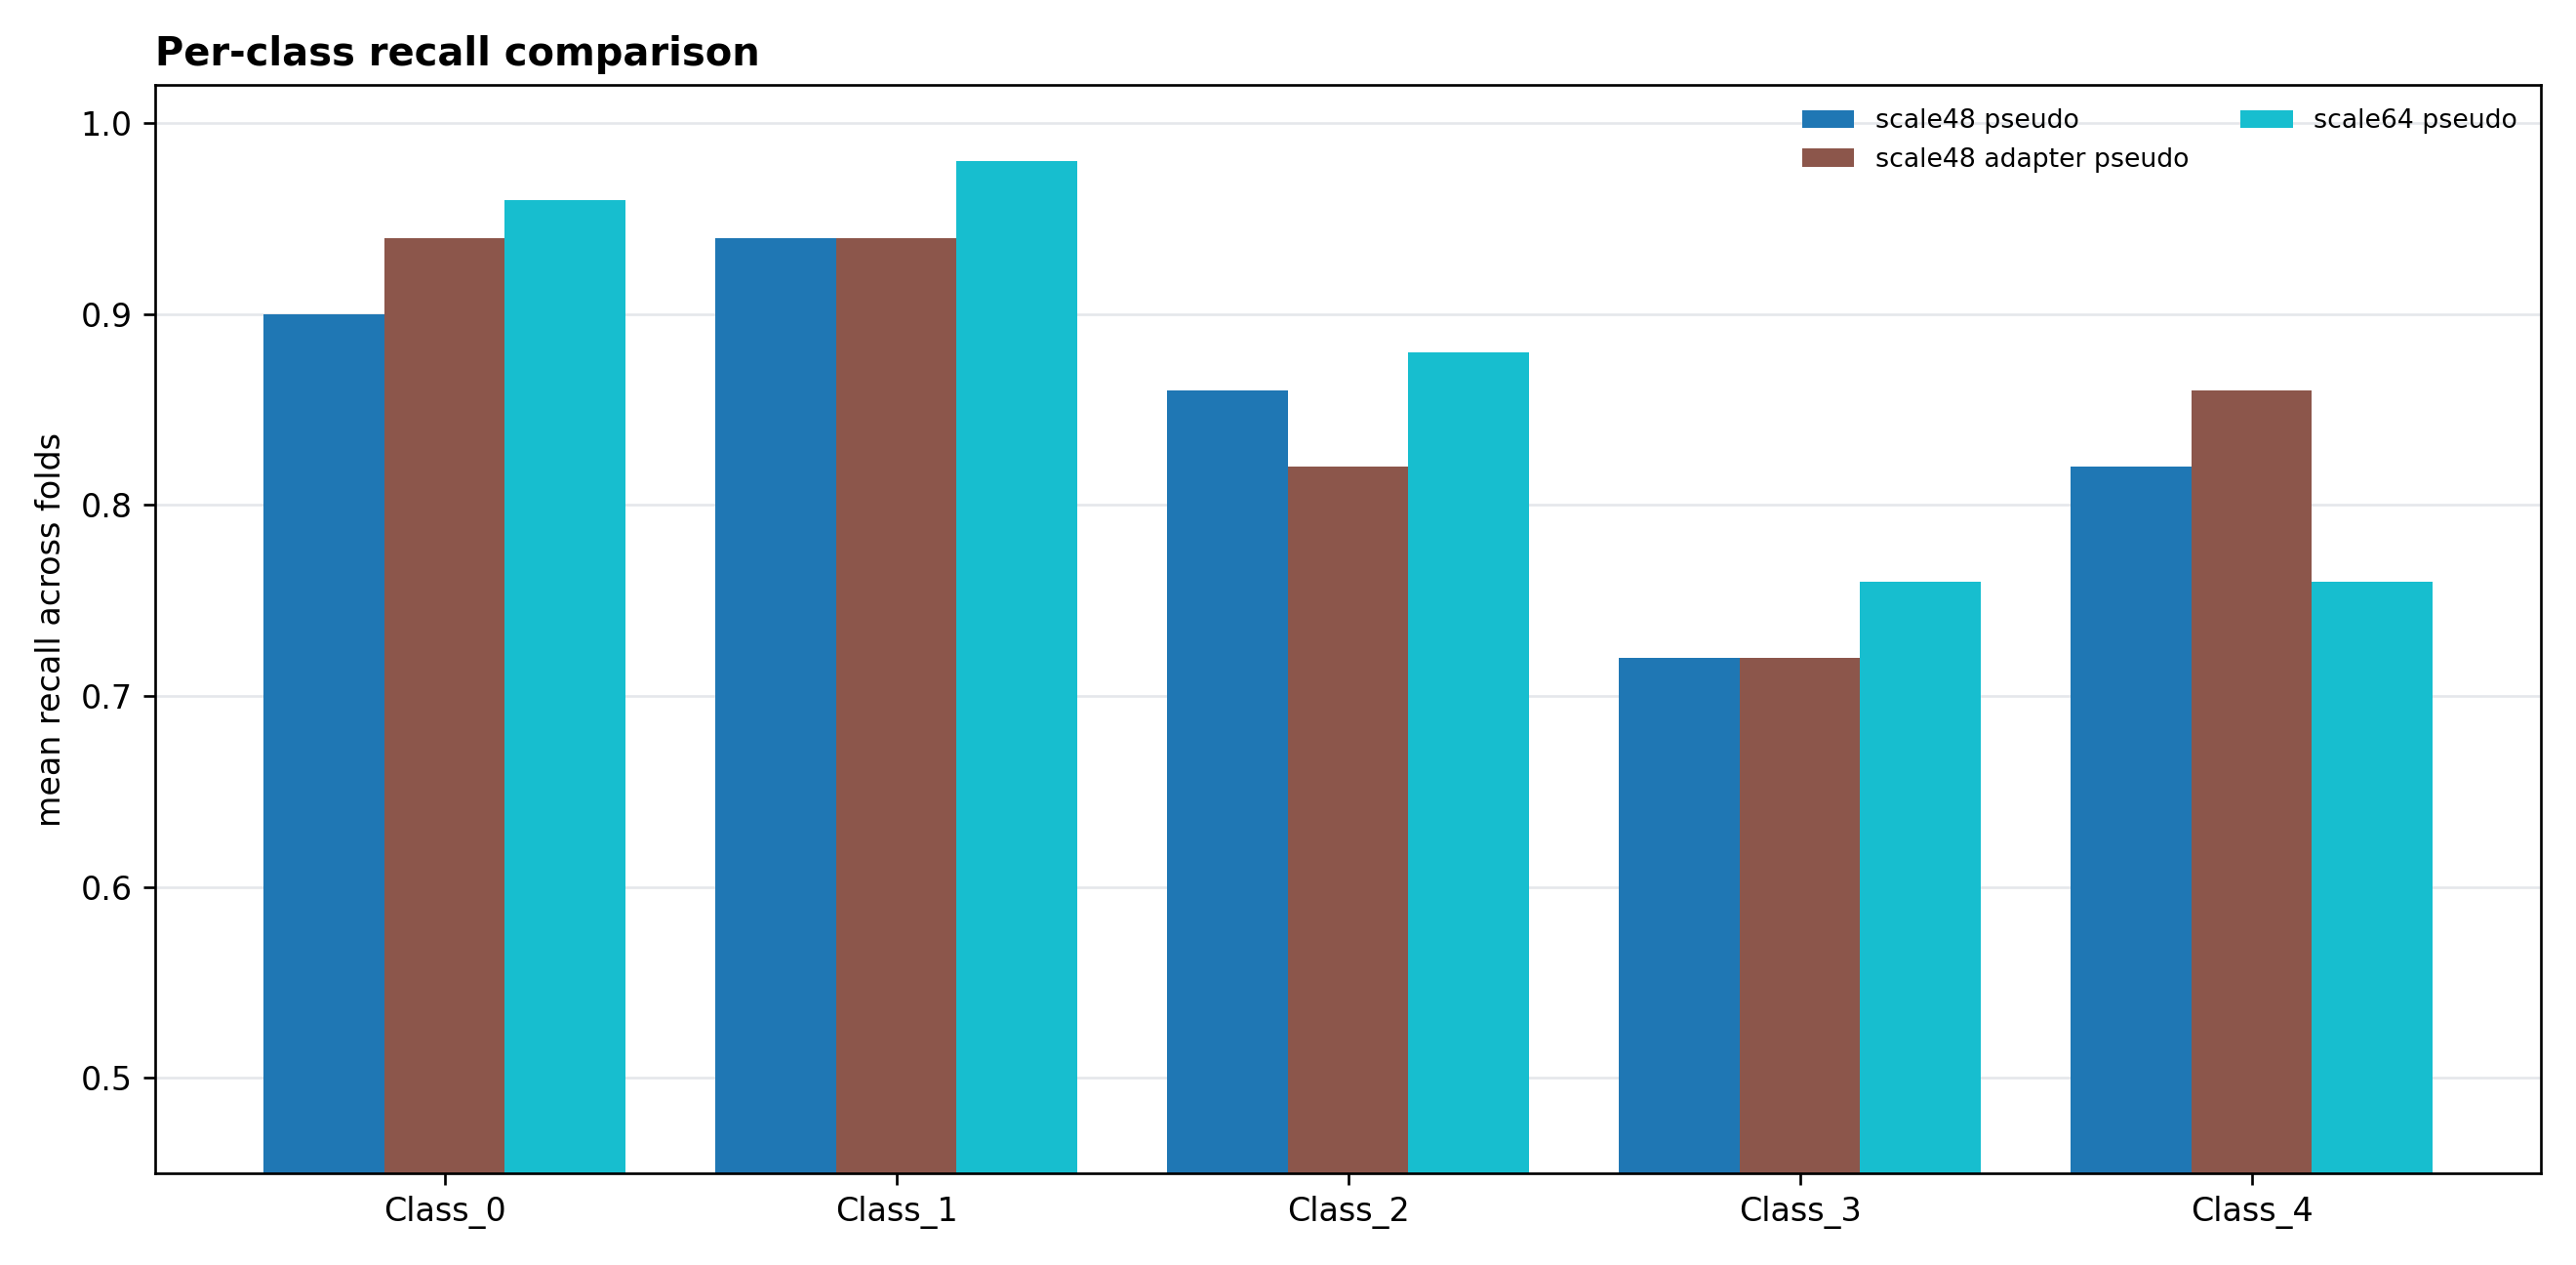
\includegraphics[width=\textwidth]{per_class_recall_comparison.png}
    \caption{最终模型与主要候选的 per-class recall 对比。最终 scale64 pseudo 模型在整体均衡性上最好，但 \(\cls{3}\) 和 \(\cls{4}\) 仍是后续改进重点。}
    \label{fig:per-class-recall}
\end{figure}

\subsection{测试集预测分布诊断}

最终提交采用 scale64 soft150 lam002 single-refit CSV，包含 61,881 行测试集预测。由于测试集没有公开标签，表 \ref{tab:test-distribution} 和图 \ref{fig:test-distribution} 只能用于分析模型输出分布，而不能用于计算真实性能。预测分布呈明显不均衡：\(\cls{0}\) 占 45.08\%，\(\cls{3}\) 和 \(\cls{4}\) 分别占 21.85\% 和 19.31\%，而 \(\cls{1}\) 仅占 4.76\%。这一结果说明 balanced pseudo-label 训练并没有把最终预测强行推向均匀分布，模型仍然根据测试图像内容形成了偏斜输出；但由于真实测试分布未知，\(\cls{0}\) 的高占比也可能带来 precision 风险。

\begin{table}[H]
    \centering
    \caption{最终提交的测试集预测分布}
    \label{tab:test-distribution}
    \small
    \begin{tabular}{lrrr}
        \toprule
        \textbf{类别} & \textbf{预测数量} & \textbf{占比} & \textbf{Top-1 中位置信心} \\
        \midrule
        \cls{0} & 27,896 & 45.08\% & 0.9319 \\
        \cls{1} & 2,947 & 4.76\% & 0.7741 \\
        \cls{2} & 5,568 & 9.00\% & 0.7214 \\
        \cls{3} & 13,523 & 21.85\% & 0.8152 \\
        \cls{4} & 11,947 & 19.31\% & 0.8038 \\
        \bottomrule
    \end{tabular}
\end{table}

置信度统计提供了进一步诊断。预测为 \(\cls{0}\) 的样本具有最高的 Top-1 中位置信心 0.9319 和最大中位 margin 0.9011，说明模型对大量 \(\cls{0}\) 预测较为确信；预测为 \(\cls{2}\) 的样本中位置信心最低，为 0.7214，中位 entropy 最高，为 0.8477，表明该类预测更接近类别边界。结合 OOF 中 \(\cls{2}\)、\(\cls{3}\)、\(\cls{4}\) 的混淆关系可以推断，测试分布中低置信样本更可能集中在形态连续、类别边界模糊的区域，而不是单纯由某一个类别造成。

\begin{figure}[H]
    \centering
    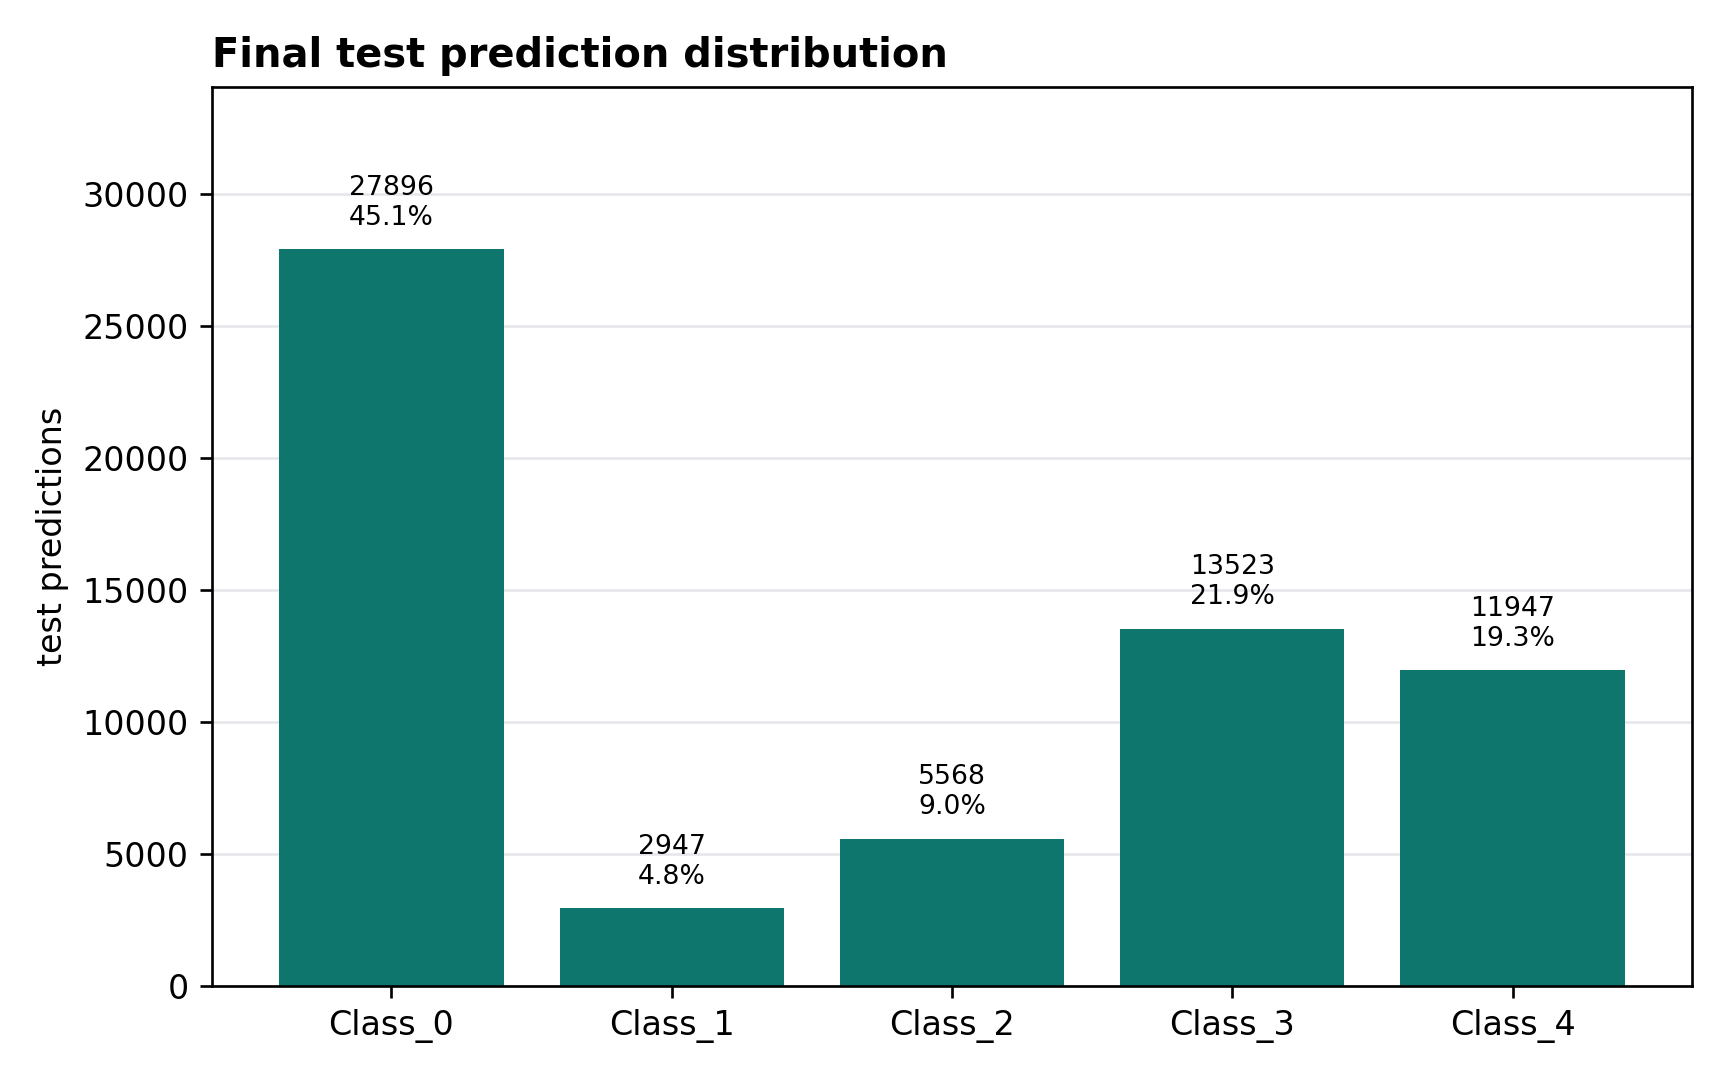
\includegraphics[width=0.82\textwidth]{test_prediction_distribution.png}
    \caption{最终提交预测分布。该图仅反映无标签测试集上的模型输出比例，不代表隐藏测试真实性能。}
    \label{fig:test-distribution}
\end{figure}

\subsection{错误案例分析}

错误分析用于判断模型失效来自低置信不确定性，还是来自高置信但错误的类别边界。图 \ref{fig:bad-cases} 展示最终模型的高置信 OOF 错误案例。错误样本主要来自 \(\cls{2}\)、\(\cls{3}\)、\(\cls{4}\)：33 个 OOF 错误案例中，\(\cls{3}\) 和 \(\cls{4}\) 各贡献 12 个，\(\cls{2}\) 贡献 6 个。最高置信错误为 \(\cls{2}\rightarrow\cls{4}\)，预测概率达到 0.9688，而真实类别概率仅为 0.0132。这类样本说明部分错误并非简单的阈值不确定，而是模型在局部纹理、核边界和染色强度相近的细胞之间形成了过强的错误判别。

\begin{figure}[H]
    \centering
    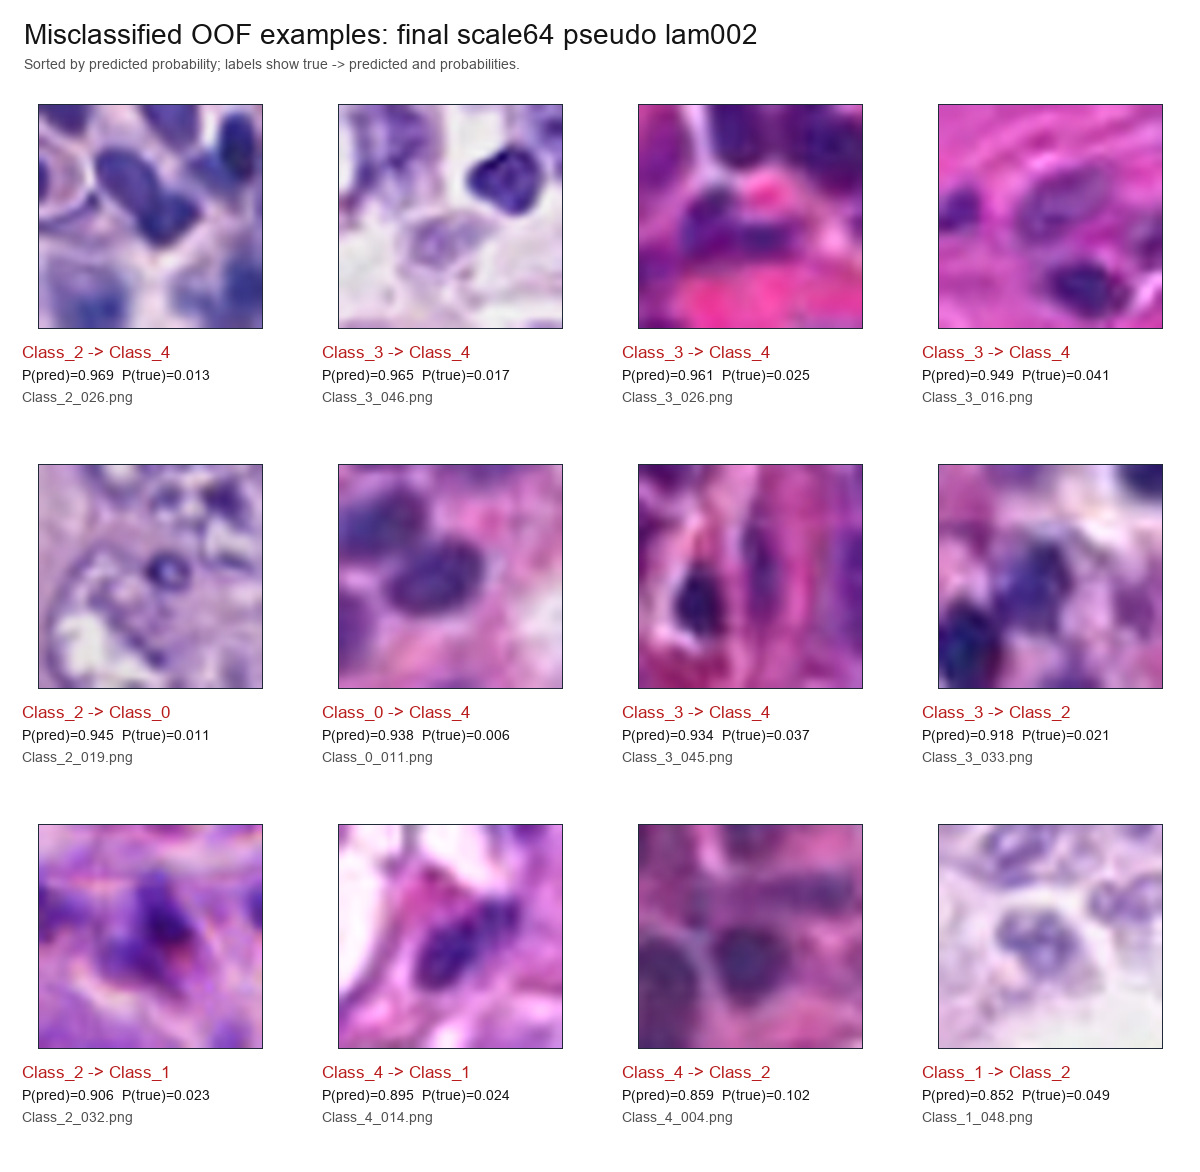
\includegraphics[width=0.86\textwidth]{misclassified_oof_examples_final_scale64_pseudo_lam002.png}
    \caption[High-confidence OOF errors]{最终模型的高置信 OOF 错误案例。错误集中在形态相近类别之间，说明模型仍存在局部纹理和弱类边界混淆。}
    \label{fig:bad-cases}
\end{figure}

持久错误对和低置信测试样本如图 \ref{fig:persistent-errors} 与图 \ref{fig:low-confidence} 所示。持久错误对表明，\(\cls{2}\rightarrow\cls{4}\)、\(\cls{4}\rightarrow\cls{2}\)、\(\cls{4}\rightarrow\cls{1}\)、\(\cls{3}\rightarrow\cls{2}\) 是出现频率较高的错误方向，前五个错误对合计 48 次，占该错误对统计中 107 次记录的 44.9\%。这些错误对的平均置信度约为 0.77--0.87，说明模型在困难类别上存在稳定的错误吸引方向。与之相对，最低置信的 500 张测试图像 Top-1 概率中位数仅为 0.3411，margin 中位数为 0.0295，entropy 中位数为 1.3855；在 5 分类问题中，这接近多类别同时竞争的状态。低置信样本的预测标签也较分散，\(\cls{3}\)、\(\cls{4}\)、\(\cls{0}\)、\(\cls{2}\)、\(\cls{1}\) 分别有 118、113、104、84、81 张。

综合来看，最终模型的错误可以分为两类：一类是高置信的形态近邻混淆，主要发生在 \(\cls{2}\)、\(\cls{3}\)、\(\cls{4}\) 之间；另一类是低置信的测试边界样本，表现为多个类别概率接近。前者提示仅靠提高分类阈值难以消除错误，后者提示 hidden 测试分布可能包含训练集中覆盖不足的形态过渡样本。因此，后续改进不应简单扩大伪标签规模，而应围绕难类边界进行更保守的伪标签筛选、类别条件阈值或细粒度 adapter 设计。

\begin{figure}[H]
    \centering
    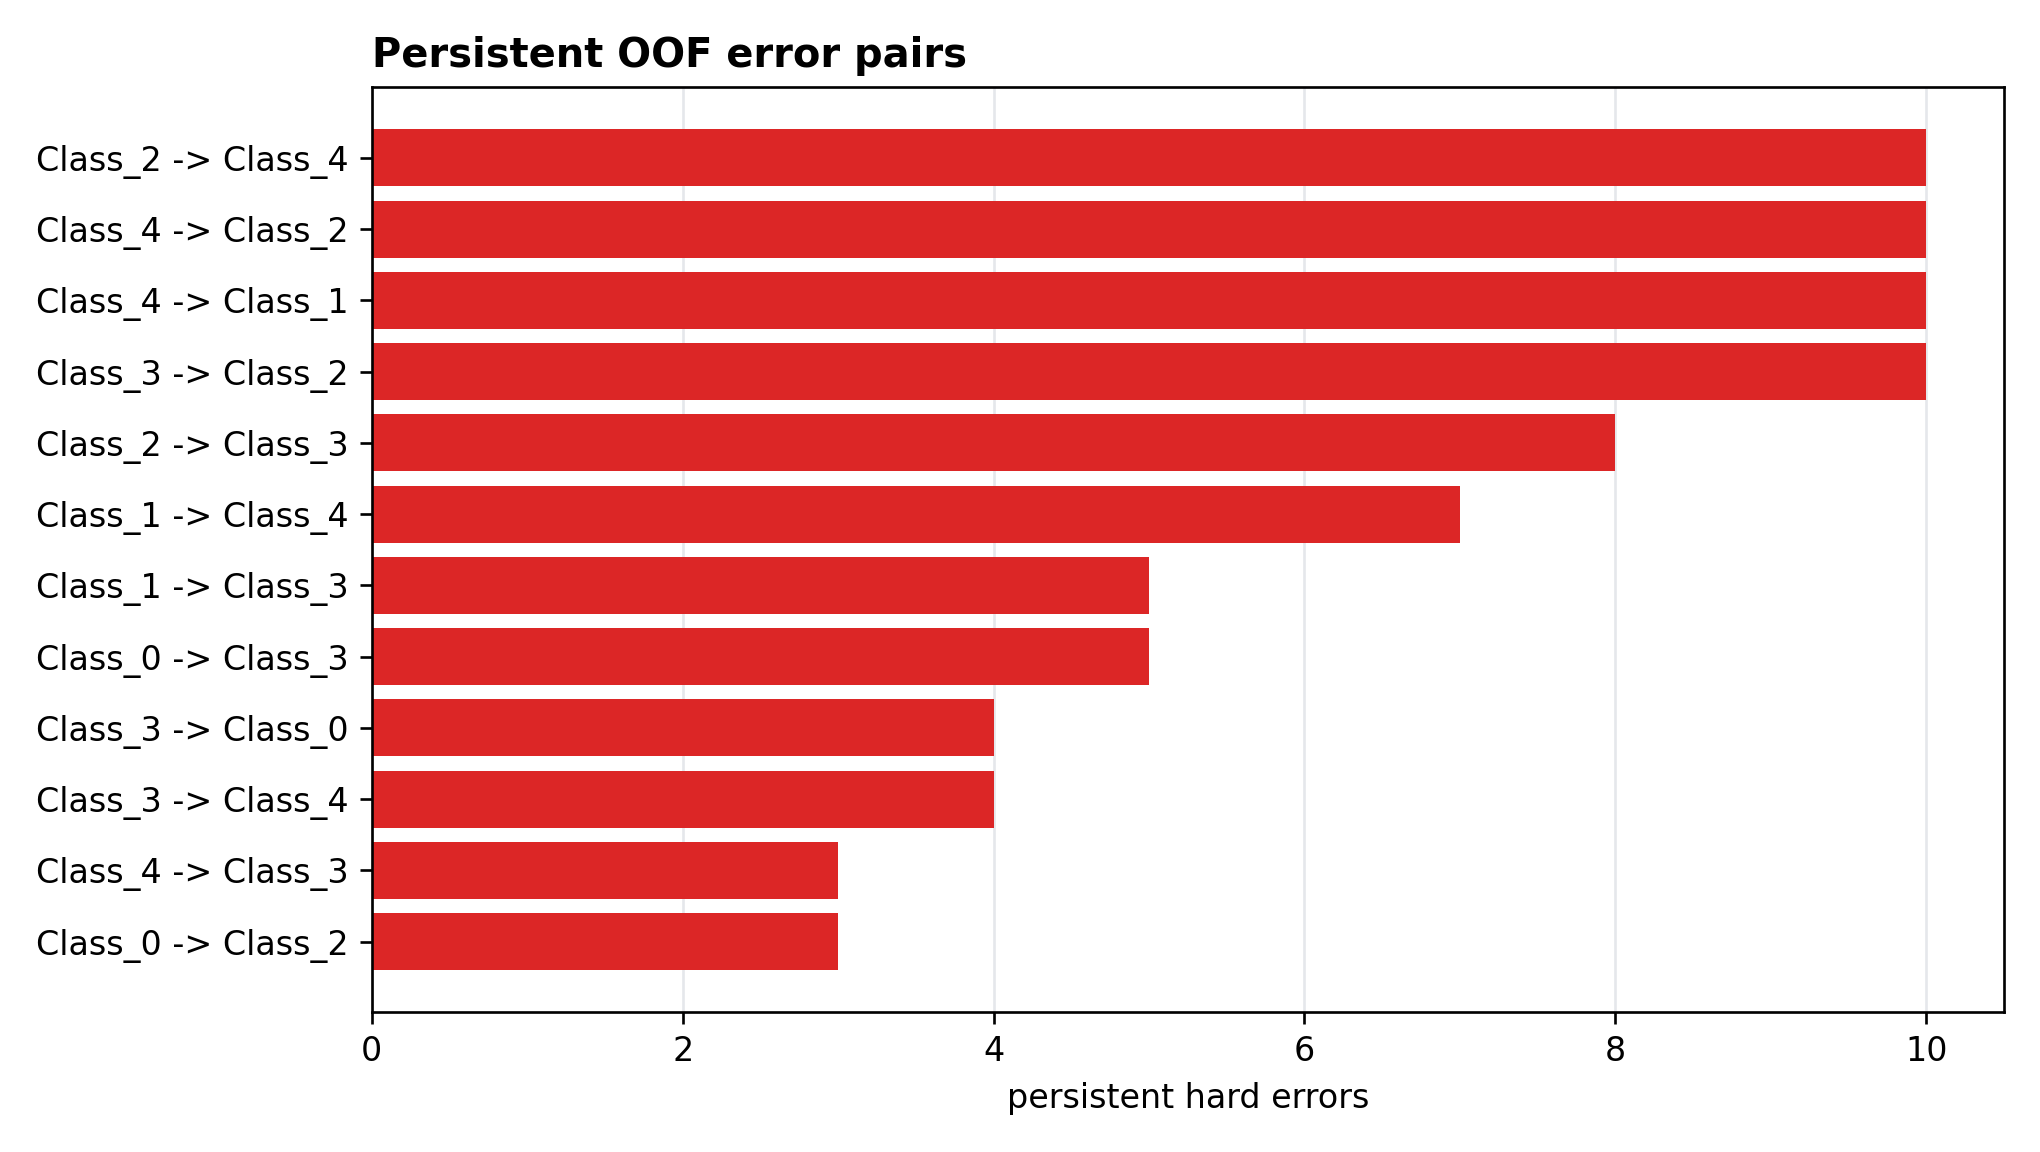
\includegraphics[width=0.9\textwidth]{persistent_error_pairs.png}
    \caption[Persistent error pairs]{持久错误对统计。相邻形态类别之间的混淆是主要误差来源。}
    \label{fig:persistent-errors}
\end{figure}

\begin{figure}[H]
    \centering
    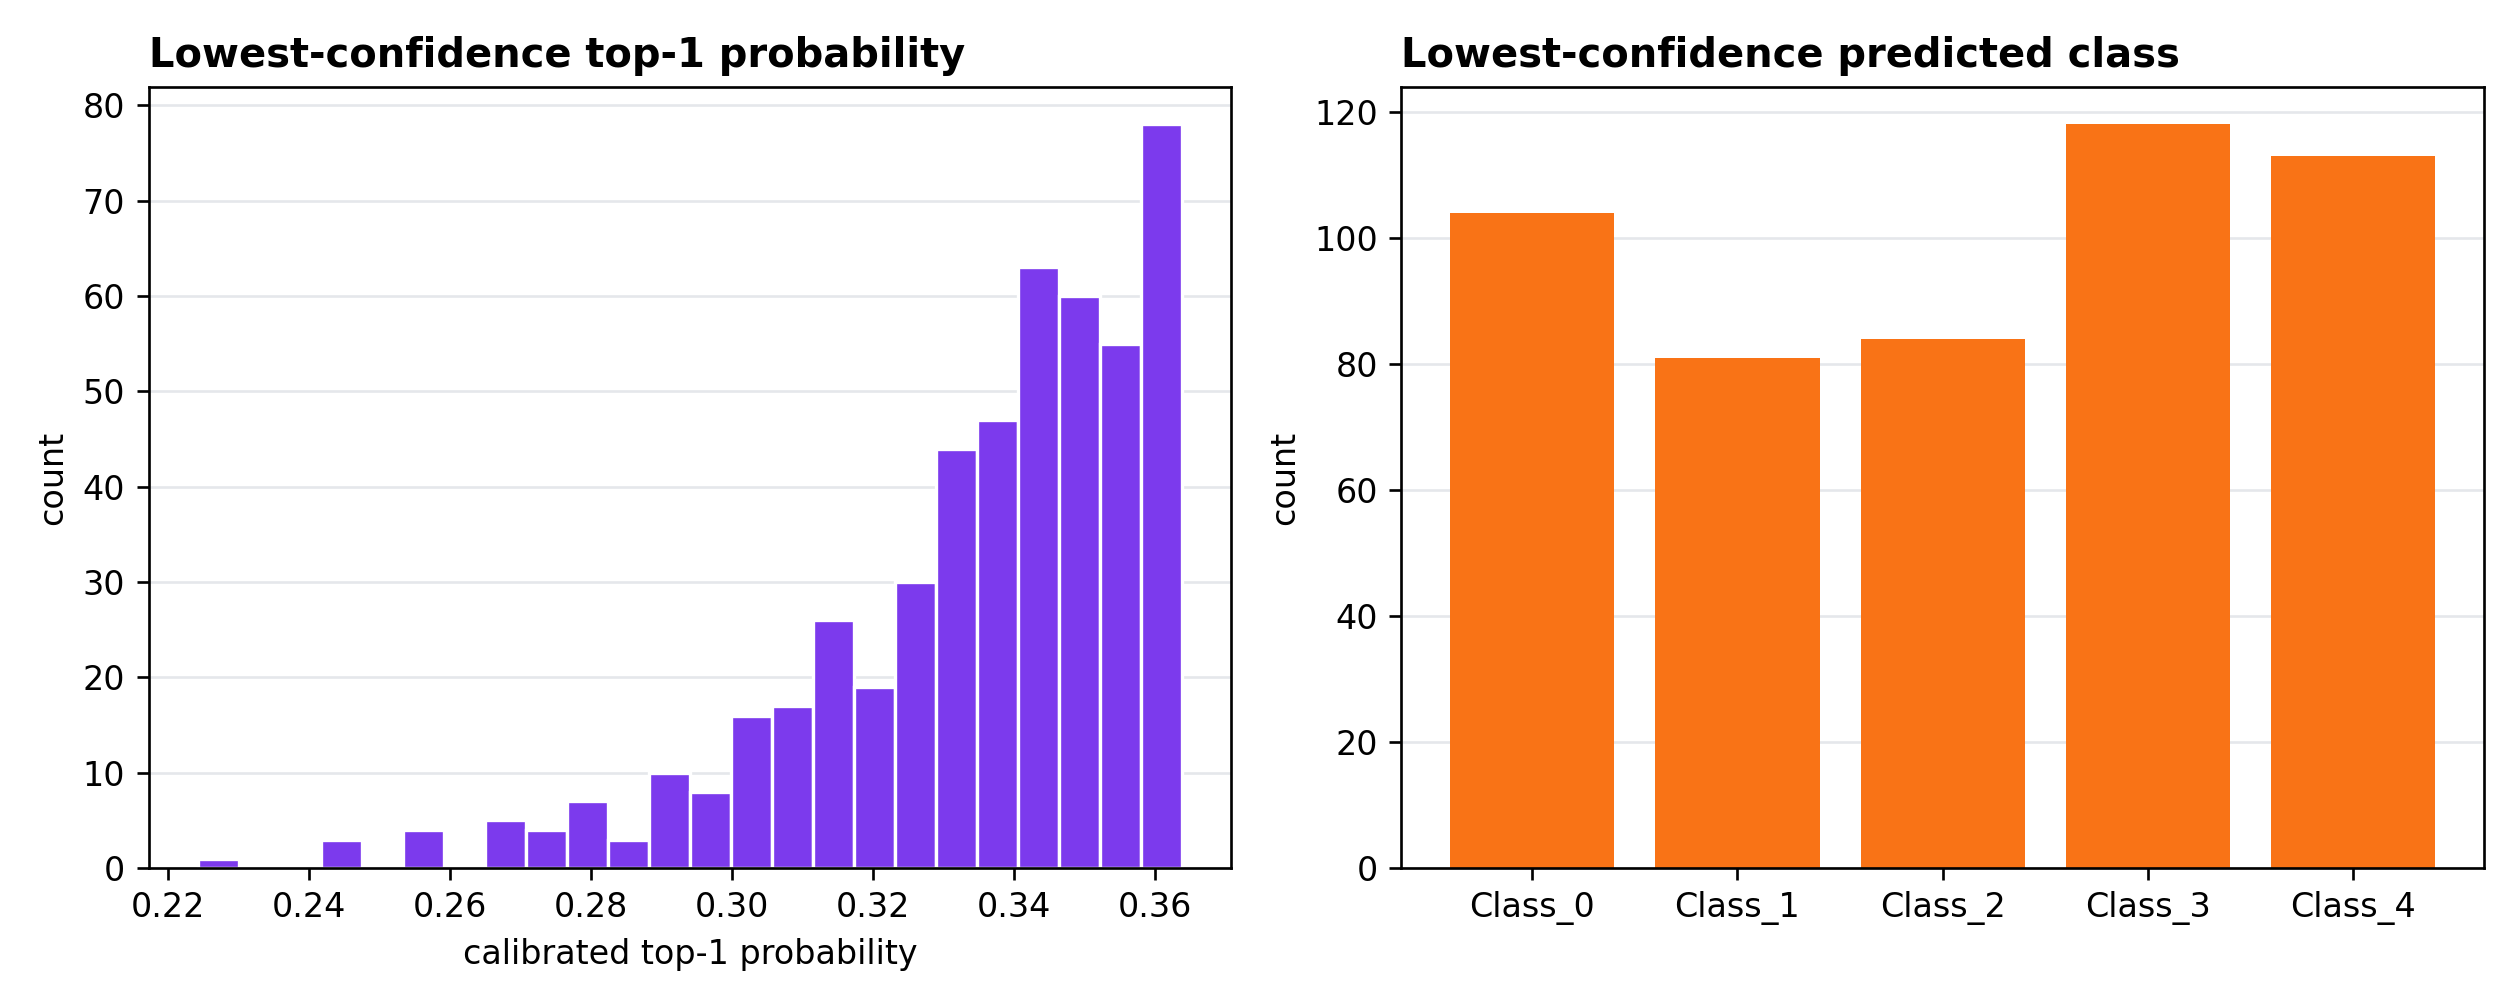
\includegraphics[width=\textwidth]{lowest_confidence_test_analysis.png}
    \caption[Low-confidence test samples]{低置信测试样本分析。低置信样本反映了测试集中的边界样本和可能的分布偏移。}
    \label{fig:low-confidence}
\end{figure}

\section{对比实验}

\subsection{整体探索路线}

对比实验按照由低复杂度基线逐步过渡到最终方法的顺序组织。这里的 Scheme01、Scheme02 和 Scheme03 是本项目内部用于区分实验路线的阶段编号：Scheme01 指冻结特征与传统分类头实验，用于估计不微调基础模型时的可达到性能；Scheme02 指参数高效微调与多 backbone 融合实验，用于检验 LoRA、adapter 和多基础模型互补性对监督性能的边际贡献；Scheme03 指伪标签自训练实验，用于在不使用外部带标签数据的前提下，利用 61,881 张无标签测试图像的分布信息。三者共同构成从“表征是否可用”到“如何适配任务”再到“如何利用无标签分布”的探索路径。

Scheme01 的作用是建立冻结特征范式下的性能基准，并识别传统 few-shot pipeline 的主要误差来源。该阶段先从 UNI2-h、CONCH、Virchow2、H-optimus-0 等病理基础模型提取冻结图像特征，再比较 multinomial logistic regression、SVM、KNN、prototype/SimpleShot、LDA shrinkage 等传统分类头；同时测试 D4 几何特征均值、训练折 D4 扩增、轻颜色扰动、四 backbone 特征拼接、FroFA fold-local feature-space augmentation、类别 bias 和层次 hard-class 分类等策略。最佳候选 selection 为 0.5934，说明冻结特征能够形成可用的初始表征，但仅训练浅层分类头不足以处理本任务的尺度错配和弱类边界。

Scheme02 进一步评估参数高效微调与多模型融合的增益。其中 Scheme02a 对单个 backbone 做参数高效微调，主要是对 attention \texttt{qkv/proj} 注入 LoRA；Scheme02b 将 UNI2-h、CONCH、Virchow2 和 H-optimus-0 组织成低容量多分支融合模型，使用投影层和分类头学习互补信息。该路线将 selection 提升到 0.7185，说明 PEFT 和多模型互补确实优于冻结特征；但是这一路线仍沿用普通 \(224\times224\) 输入视图，并没有系统解决 \(32\times32\) 单细胞图像与病理 foundation model 预训练尺度之间的错配。随后进入 UNI2-h 尺度校准和伪标签实验，是因为前两阶段已经显示：模型容量和 backbone 数量并非唯一限制，输入视图本身可能是更基础的制约因素。

表 \ref{tab:route-comparison} 汇总了关键探索节点。一个 selection 为 0.9440 的异常记录未纳入主结论，因为其 split 和数据可比性没有在最终报告链路中重新核验；下表只保留可追溯到正式 OOF/CV 结果、且与最终方法可比较的实验。

\begin{table}[H]
    \centering
    \caption{主要探索阶段、实验内容与关键结论}
    \label{tab:route-comparison}
    \small
    \resizebox{\textwidth}{!}{
    \begin{tabular}{L{2.6cm}L{6.8cm}rrL{6.5cm}}
        \toprule
        \textbf{阶段} & \textbf{具体实验内容} & \textbf{Macro-F1} & \textbf{Selection} & \textbf{结论} \\
        \midrule
        Scheme01：冻结特征基线 & 多病理 backbone 冻结特征；logreg/SVM/KNN/prototype 等分类头；D4、轻颜色扰动、特征拼接与 FroFA。 & 0.5907 & 0.5934 & 建立了冻结特征基准，但浅层 head 难以充分适配单细胞尺度和弱类边界。 \\
        Scheme02：PEFT 与融合 & 单 backbone LoRA 微调；UNI2-h/CONCH/Virchow2/H-optimus-0 四分支低容量融合。 & 0.7170 & 0.7185 & PEFT 与多模型互补带来增益，但仍未处理输入尺度与预训练视野不一致的问题。 \\
        早期 fusion pseudo & 使用 Scheme02 fusion teacher 的测试伪标签策略，伪标签集中于易类，\(\cls{3}\)/\(\cls{4}\) 没有伪标签。 & 0.7159 & 0.7160 & 不均衡伪标签没有超过 supervised fusion，说明教师模型可靠性和类别覆盖都必须受控。 \\
        UNI scale64 supervised & 单 UNI2-h，\texttt{CenterScalePad(scale64)}，rsLoRA 与难类权重，仅使用 250 张真实标签。 & 0.7500 & 0.7510 & 尺度校准后的单模型超过早期多模型融合，提示输入视图是关键变量。 \\
        UNI scale64 pseudo-250 & scale64 teacher 选取 250 张均衡伪标签，低权重伪标签损失。 & 0.8227 & 0.8234 & 当 teacher 已经过尺度校准且伪标签保持类别覆盖时，无标签分布开始提供正收益。 \\
        UNI scale64 soft150 & 每类 150 张均衡软伪标签，共 750 张；soft label 与 \(\lambda_{\mathrm{pseudo}}=0.002\)。 & 0.8662 & 0.8671 & 最终方案在本地 OOF 上取得最高可比结果，收益来自尺度校准、PEFT 和受控伪标签的组合。 \\
        \bottomrule
    \end{tabular}
    }
\end{table}

\subsection{尺度消融实验}

尺度消融用于检验输入视图是否是影响迁移效果的独立因素。实验保持 backbone、rsLoRA 注入位置、难类权重、fold 划分和训练策略不变，仅改变 \(32\times32\) 原图在 \(224\times224\) 画布中的有效显示尺度。由于 UNI2-h 使用 ViT-H/14 结构，patch size 为 14，因此输入尺度实际上决定了细胞横向覆盖的 patch 数量：full224 约覆盖 16 个 patch，scale32 约覆盖 2.3 个 patch，scale48 约覆盖 3.4 个 patch，scale64 约覆盖 4.6 个 patch，scale80 约覆盖 5.7 个 patch。这个变量直接影响模型看到的是“铺满视野的放大细胞”，还是“位于病理视野中心的局部目标”。

\begin{table}[H]
    \centering
    \caption{输入尺度消融实验}
    \label{tab:scale-ablation}
    \small
    \resizebox{\textwidth}{!}{
    \begin{tabular}{lrrrrL{6.0cm}}
        \toprule
        \textbf{输入视图} & \textbf{约 patch 跨度} & \textbf{Macro-F1} & \textbf{Balanced Acc.} & \textbf{Selection} & \textbf{解释} \\
        \midrule
        full224 & 16.0 & 0.7072 & 0.7080 & 0.7076 & 直接拉伸到整幅画布，细胞结构被过度放大，插值纹理也被同步放大。 \\
        scale32 & 2.3 & 0.7154 & 0.7120 & 0.7137 & 接近原始尺度，但目标在 token 网格中覆盖过少，形态信息表达不足。 \\
        scale48 & 3.4 & 0.7709 & 0.7680 & 0.7694 & 监督消融中最高，说明中等局部目标尺度更适合 UNI2-h 表征。 \\
        scale64 & 4.6 & 0.7500 & 0.7520 & 0.7510 & 略低于 scale48，但后续 teacher、伪标签、CV 与提交链路完整闭环。 \\
        scale80 & 5.7 & 0.7384 & 0.7400 & 0.7392 & 继续放大后回落，说明增大细胞占比并非单调收益。 \\
        \bottomrule
    \end{tabular}
    }
\end{table}

\begin{figure}[H]
    \centering
    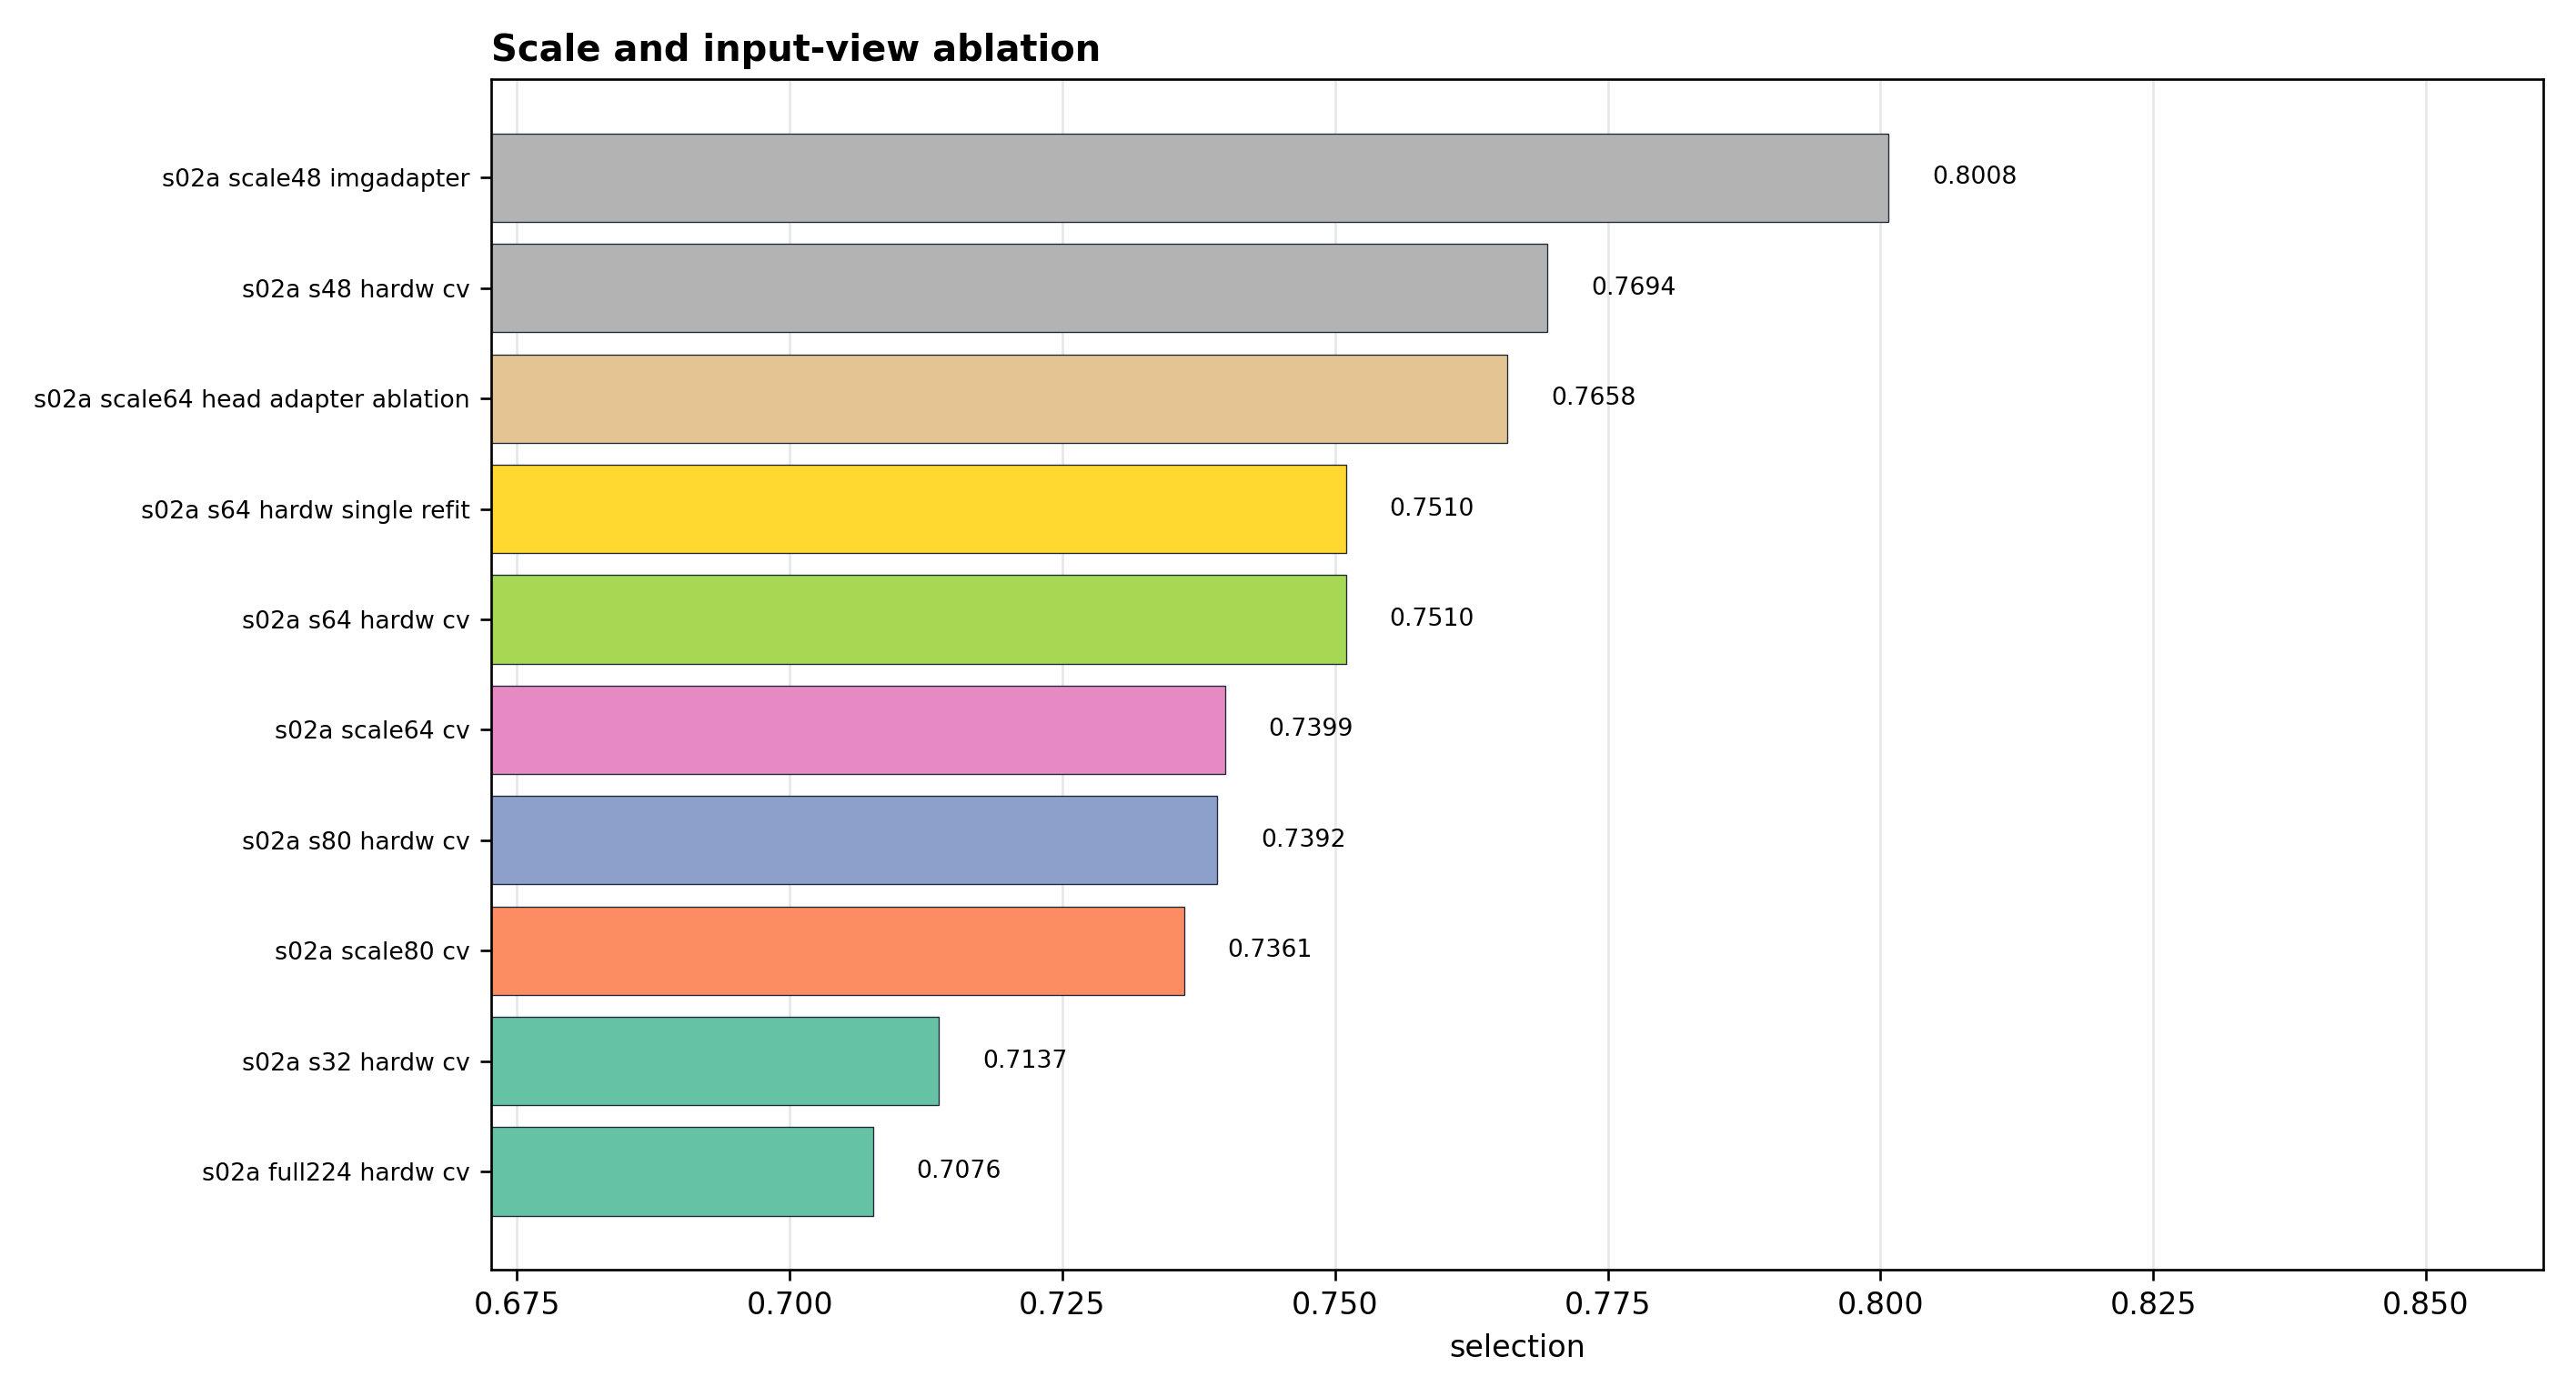
\includegraphics[width=\textwidth]{scale_ablation_selection.png}
    \caption{输入尺度消融。CenterScalePad 相比 full resize 取得更高 selection，支持主要收益来自尺度校准而不是单纯改变模型容量的判断。}
    \label{fig:scale-ablation}
\end{figure}

尺度结果显示，直接 full resize 的 selection 为 0.7076，而 scale48 与 scale64 分别达到 0.7694 和 0.7510。由于这些实验只改变输入视图，不改变 backbone 或可训练参数规模，因此差异更合理地归因于输入尺度与预训练表征之间的匹配程度。scale32 只比 full224 高 0.0061，说明“不过度放大”本身并不足够；scale80 低于 scale64，也说明继续增大细胞占比会破坏局部目标假设。换言之，有效策略不是简单地让图像更大或更小，而是在 ViT token 网格中为细胞保留合适的局部跨度。

最终提交采用 scale64 而不是监督消融中分数更高的 scale48，原因在于最终方法需要同时考虑 teacher 生成、伪标签筛选、CV 选择和 full-refit 提交的完整链路。scale48 在纯监督 OOF 中表现更好，但其后续自伪标签闭环与 adapter 变体没有超过 scale64 soft150 lam002；相反，scale64 已完成 teacher、balanced soft pseudo、5-fold OOF 与 single-refit 的一致验证。因此，本报告将 scale48 视为有潜力的后续方向，而不把单一监督消融结果直接替代最终提交方案。

\subsection{伪标签与 adapter 消融}

伪标签实验的核心问题是：无标签测试图像能否提供额外分布信息，以及这种信息在何种条件下不会被教师模型预测噪声破坏。早期 fusion pseudo 结果给出了反例。Scheme02 fusion teacher 的未均衡筛选策略只选择了 210 张伪标签，其中 \(\cls{0}=100\)、\(\cls{1}=80\)、\(\cls{2}=30\)，\(\cls{3}\) 和 \(\cls{4}\) 为 0；由该伪标签集训练得到的 student 模型 selection 为 0.7160，低于 supervised fusion 的 0.7185。这说明在类别覆盖不足时，伪标签会强化容易类别的决策区域，而不能改善 macro-F1 和 balanced accuracy 所关注的弱类表现。

在尺度校准后的 UNI2-h 上，伪标签开始产生稳定收益。scale64 supervised 的 selection 为 0.7510；加入 250 张均衡伪标签后，selection 提升到 0.8234。随后将伪标签扩展为 soft100（每类 100 张，共 500 张）得到 0.8392；soft150（每类 150 张，共 750 张）在 \(\lambda=0.001\)、0.0015、0.002 下分别达到 0.8554、0.8596、0.8671。这个序列说明收益不是来自简单增加无标签样本数量，而是来自三个约束共同作用：teacher 本身经过尺度校准，伪标签按类别均衡抽取，soft label 与低 \(\lambda_{\mathrm{pseudo}}\) 降低了错误伪标签对监督信号的覆盖。

\begin{figure}[H]
    \centering
    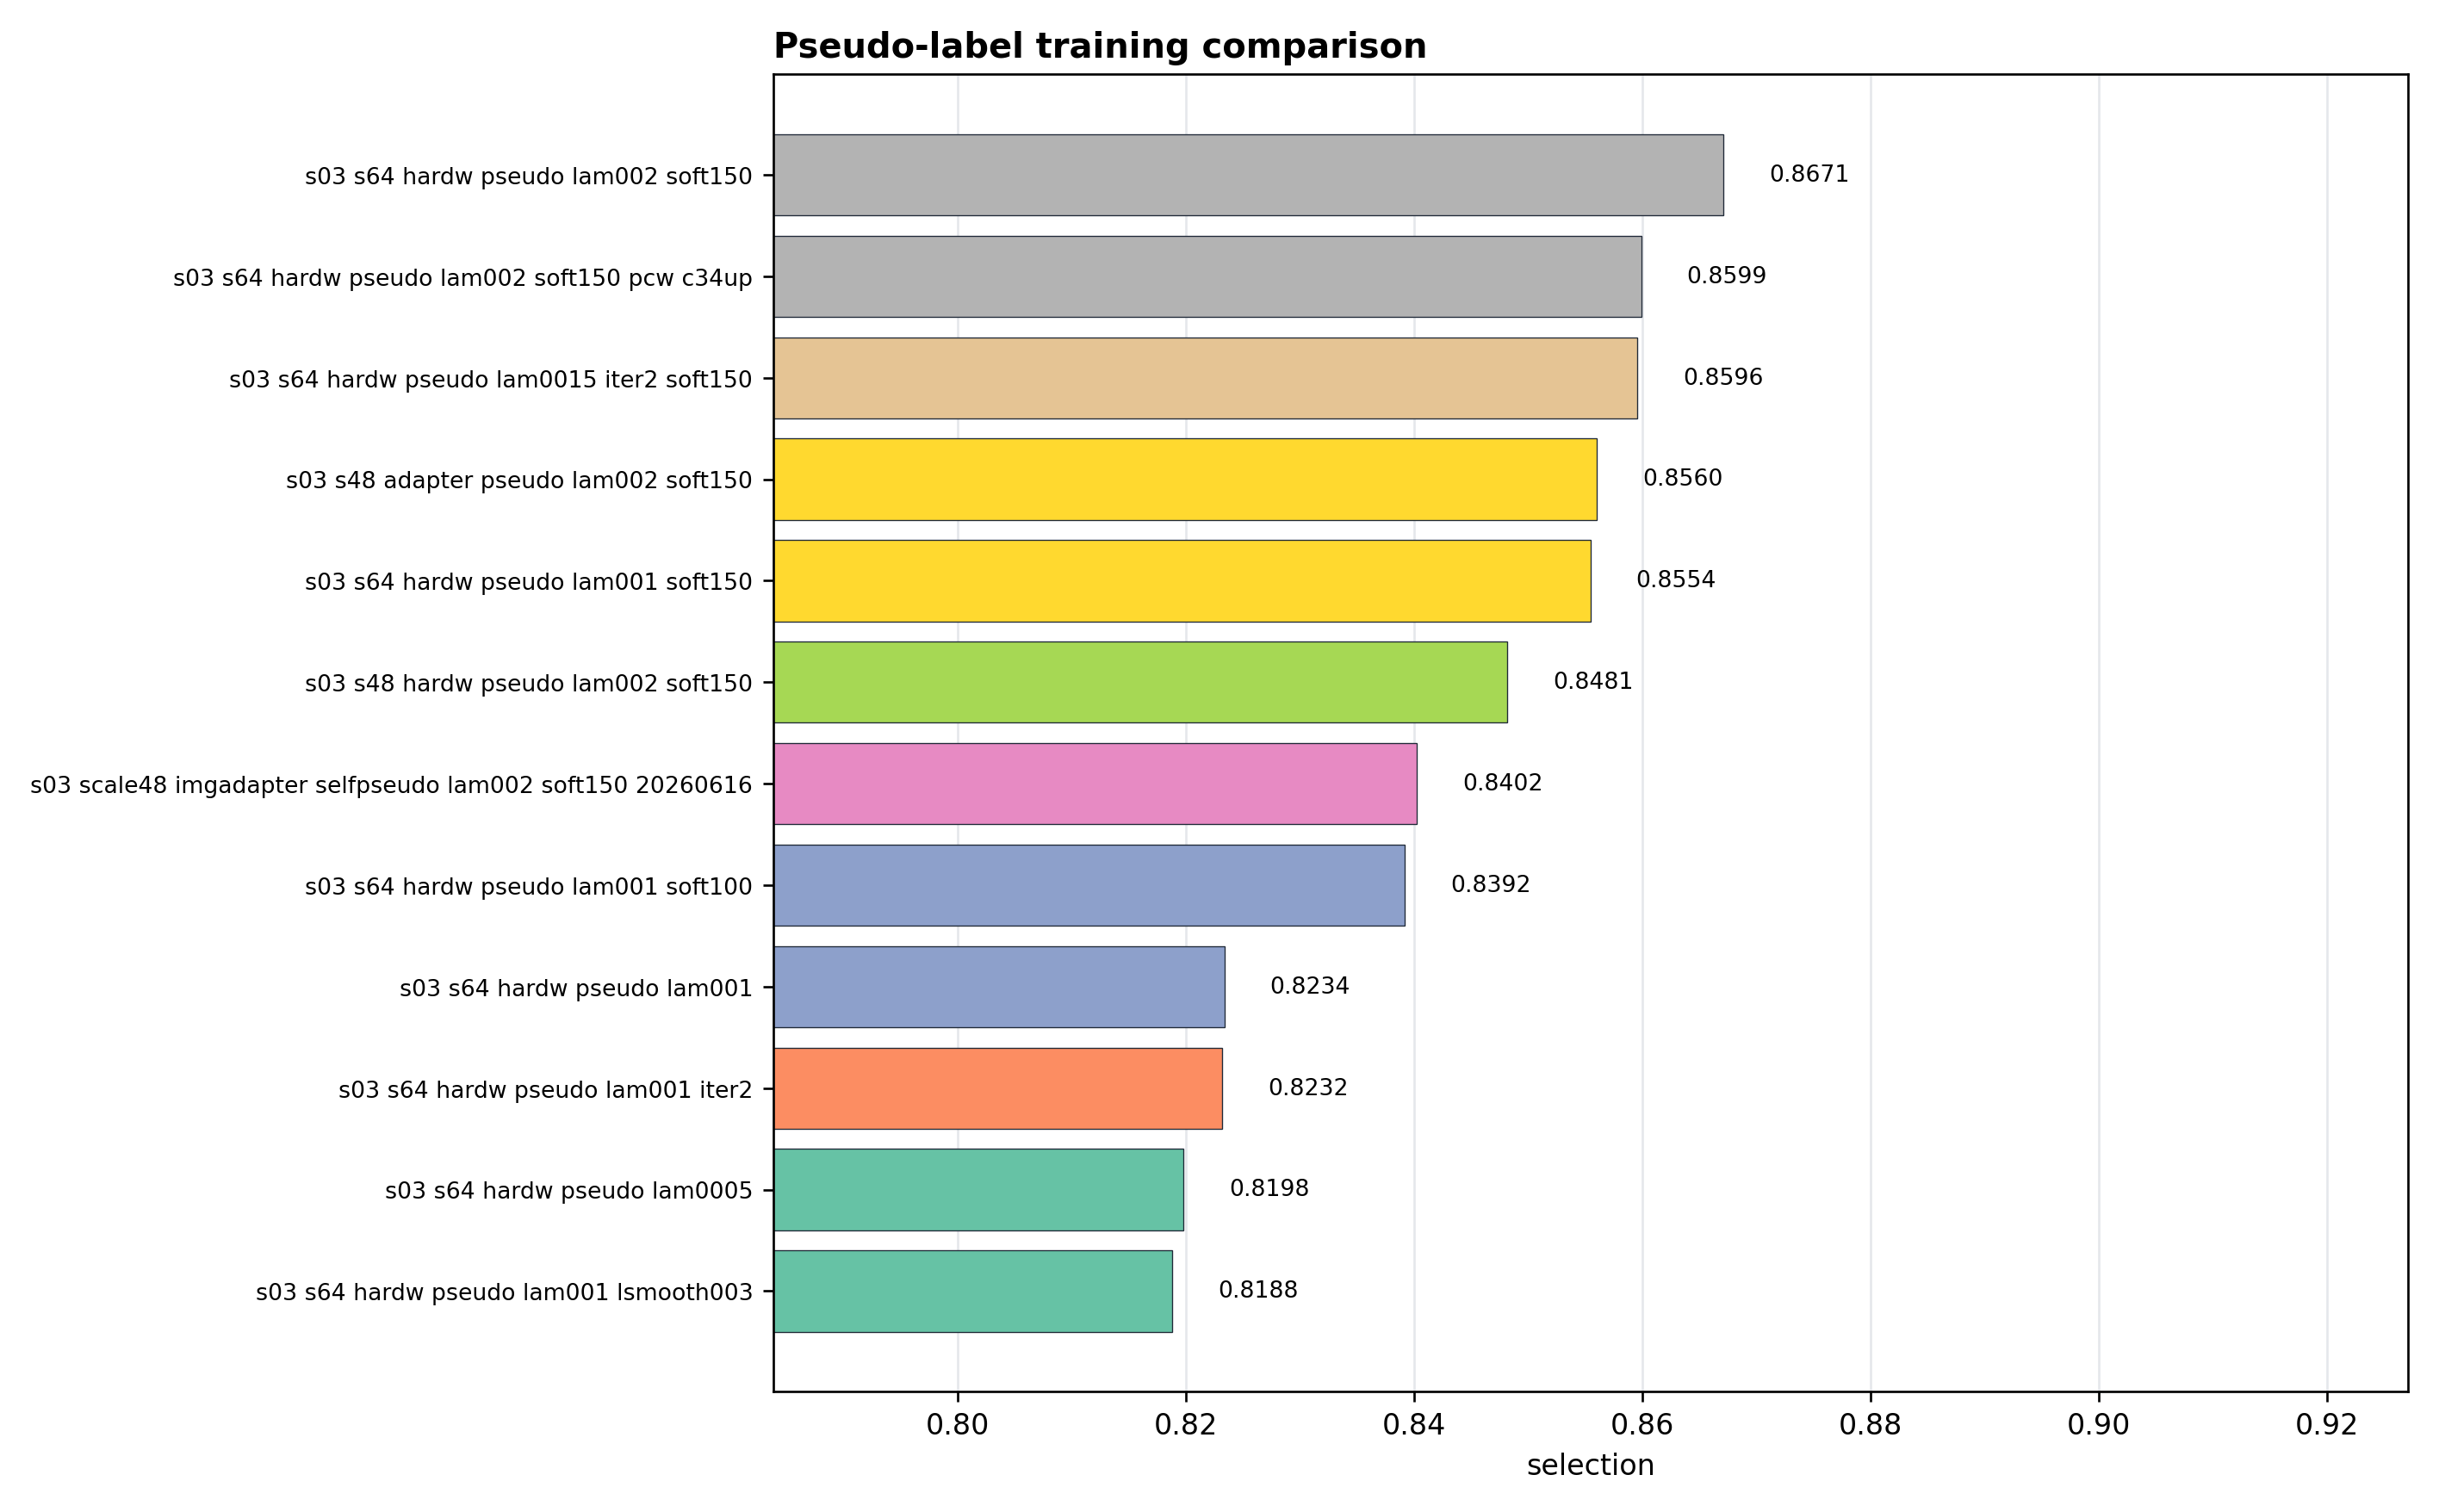
\includegraphics[width=\textwidth]{pseudo_training_selection.png}
    \caption{伪标签训练消融。balanced soft150 与 \(\lambda=0.002\) 在本地 OOF 中取得最高 selection。}
    \label{fig:pseudo-ablation}
\end{figure}

伪标签权重的结果也体现了少样本半监督训练的边界。对于 250 张伪标签，\(\lambda=0.001\) 达到 0.8234，而 \(\lambda=0.002\) 降至 0.8118；这说明当伪标签规模较小且仍包含教师模型预测噪声时，提高损失权重可能过早改变决策边界。对于 750 张 balanced soft pseudo，\(\lambda=0.002\) 反而高于 \(\lambda=0.001\)，说明在类别覆盖更完整、标签为 soft distribution、样本采用秩次权重后，模型可以承受略强的测试分布约束。最终 \(\lambda=0.002\) 的选择因此并非单独由超参数搜索决定，而是与伪标签池质量和权重设计共同成立。

图 \ref{fig:adapter-ablation} 展示 adapter 与分类头结构的补充消融。image adapter 是置于输入端的轻量 residual convolution，其目的是在进入 UNI2-h 前对低分辨率细胞图像做小幅局部校正；MLP head 则试图用更复杂的分类边界替代线性头。scale48 image adapter 在监督 CV 中将 selection 从 0.7694 提升到 0.8008，说明对输入局部纹理做轻量适配有一定价值；加入 soft150 pseudo 后达到 0.8560，但仍低于最终 scale64 soft150 lam002 的 0.8671。scale64 的 head/adapter 消融中，image adapter 最好为 0.7658，MLP head 为 0.7399，image adapter + MLP 为 0.7427，均没有超过相同尺度下的最终伪标签方案。

这些结果表明，结构复杂度本身不是最终收益的主要来源。adapter 可以改善某些监督设置下的输入适配，特别是 scale48；但当伪标签 teacher、输入尺度和最终提交链路不完全一致时，adapter 的增益会变得不稳定。相反，最终 scale64 路线虽然监督消融不是最高，但在 teacher 生成、balanced soft pseudo 和 full-refit 上保持一致，因而形成了更可复现的闭环。由此可见，本项目的有效改进顺序是先校准输入尺度，再用保守 PEFT 适配基础模型，最后在类别均衡和低权重约束下引入软伪标签；单独增加 head 或 adapter 复杂度不足以替代这一链路。

\begin{figure}[H]
    \centering
    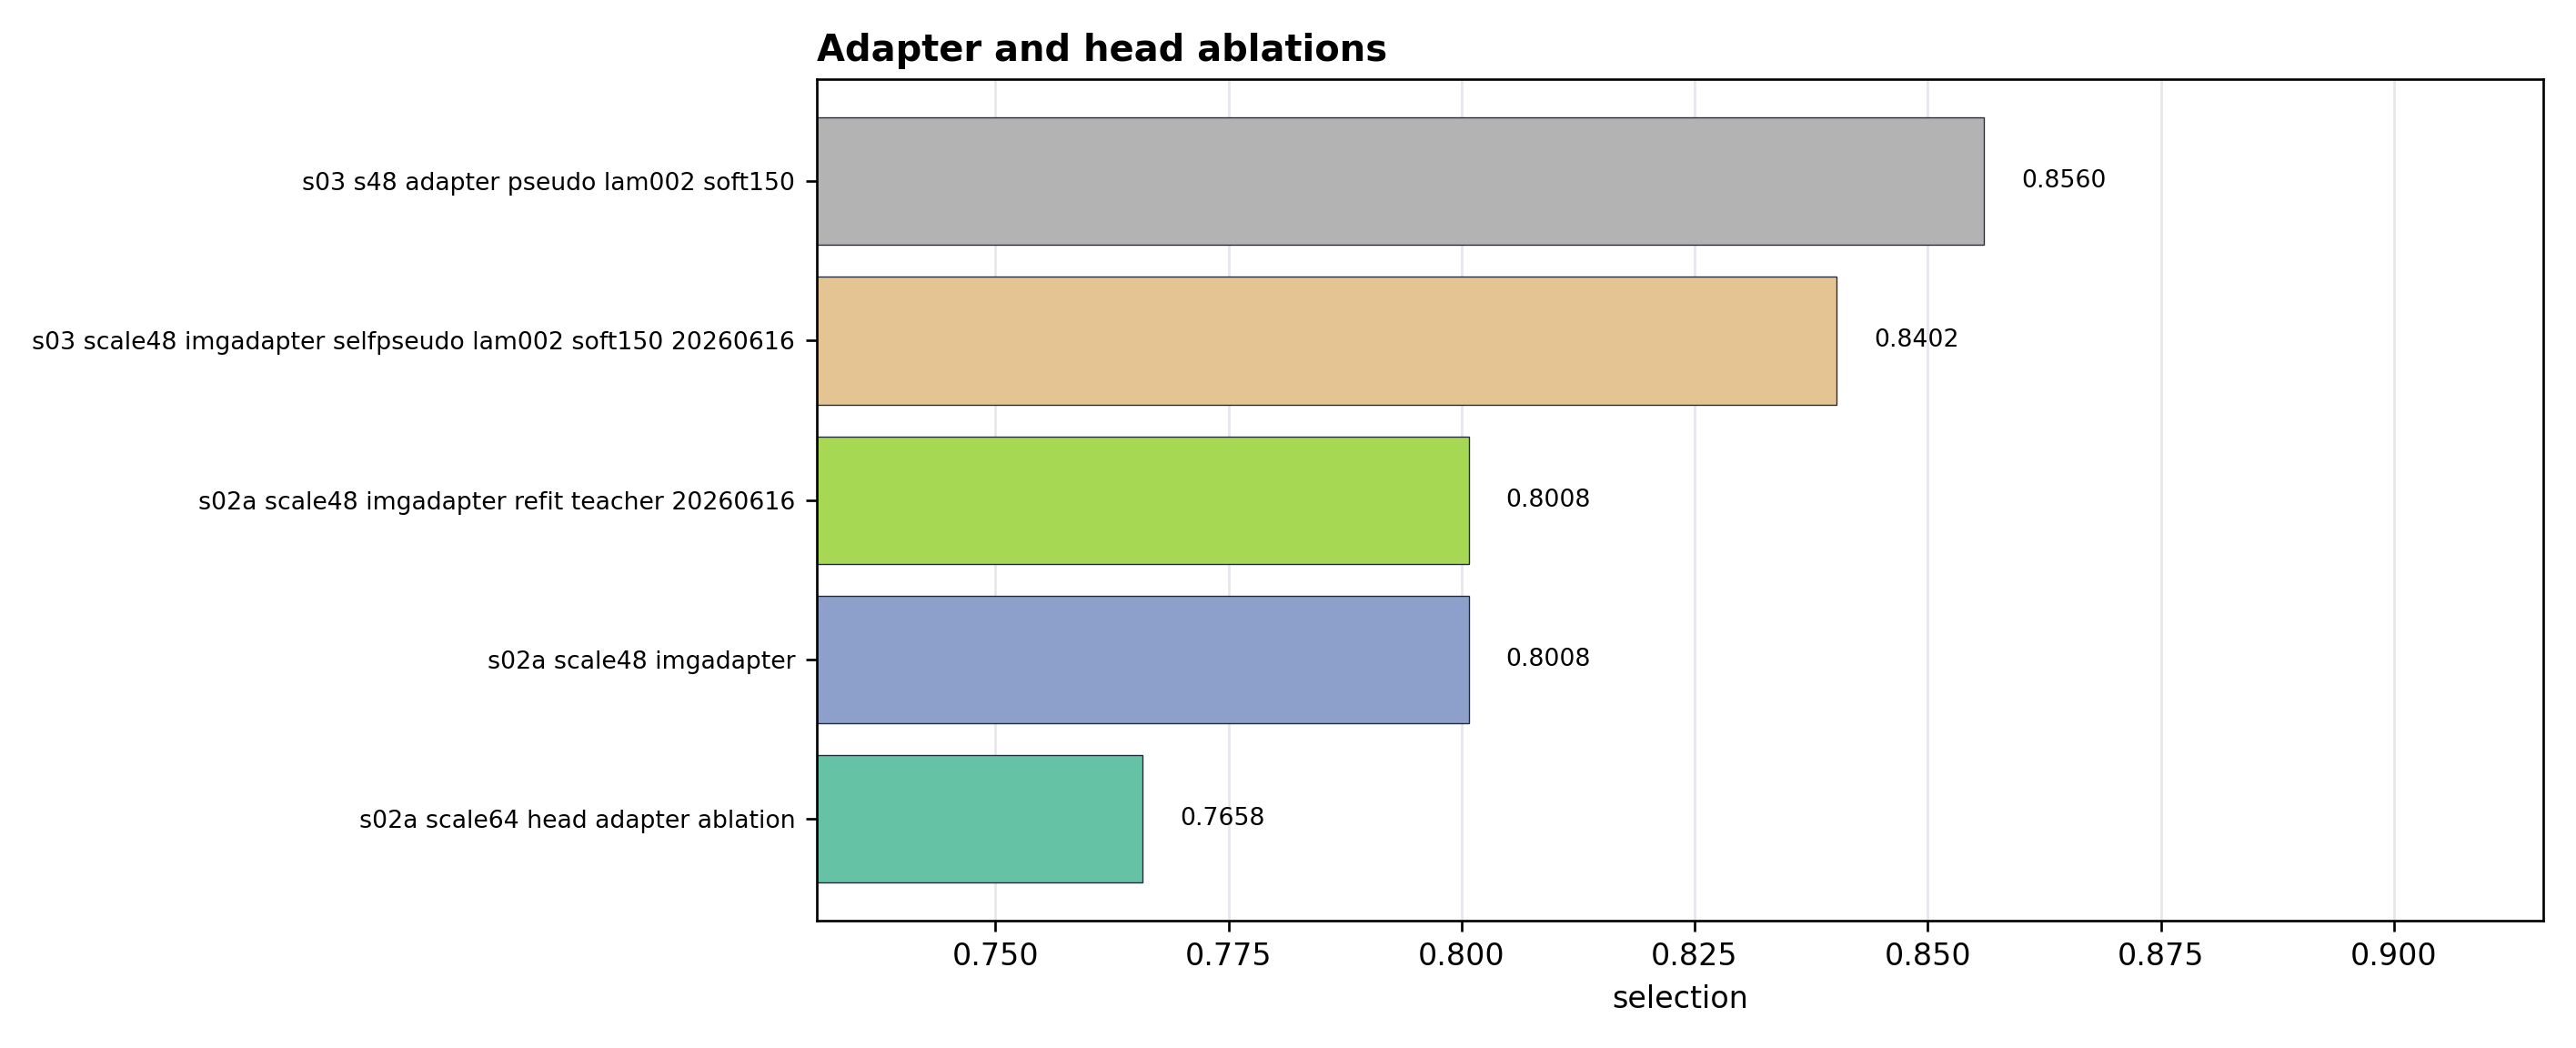
\includegraphics[width=\textwidth]{adapter_ablation_selection.png}
    \caption{head 与 image adapter 消融。轻量 image adapter 在部分设置下取得增益，但未超过最终 scale64 soft150 lam002；复杂 MLP head 没有被结果支持。}
    \label{fig:adapter-ablation}
\end{figure}

\section{最终挑战 (Final Test Challenge)}

\subsection{测试集表现}

最终外部评测采用 full-250 single-refit 模型在 61,881 张无标签测试图像上的单模型预测结果。该结果由同一套 scale64 预处理、UNI2-h backbone、rsLoRA 适配层和线性分类头产生，未使用 prediction-level TTA 或模型集成。教师/平台反馈结果如表 \ref{tab:hidden-score} 所示。本地 5-fold OOF 分数用于内部模型选择，隐藏测试分数用于外部泛化评估；二者对应的数据规模、类别分布和统计对象不同，因此在报告中分别列出。

\begin{table}[H]
    \centering
    \caption{最终隐藏测试反馈}
    \label{tab:hidden-score}
    \begin{tabular}{lc}
        \toprule
        \textbf{指标} & \textbf{结果} \\
        \midrule
        Hidden F1 & 0.5889 \\
        Hidden Recall & 0.7202 \\
        课堂排名 & 班级前 5 \\
        本地 5-fold OOF selection & 0.8671 \\
        \bottomrule
    \end{tabular}
\end{table}

隐藏测试反馈呈现出一个重要现象：Recall 为 0.7202，而 F1 为 0.5889。由于 F1 同时受到 precision 和 recall 影响，在 recall 相对较高而 F1 明显较低的情况下，一种与指标关系一致的解释是模型在隐藏测试集上覆盖了较多正例，但同时产生了较多 false positive，导致精度项限制了最终 F1。平台未公开类别级混淆矩阵，因此不能直接判断哪一个类别贡献了主要误差；但本地证据提供了可解释的风险来源。首先，OOF 中 \(\cls{3}\) 与 \(\cls{4}\) 的 recall 均为 0.76，且 33 个 OOF 错误中有 30 个来自 \(\cls{2}\)、\(\cls{3}\)、\(\cls{4}\)，说明困难边界集中在形态相近类别之间。其次，最终提交的预测分布并不均匀：\(\cls{0}\) 占 45.08\%，\(\cls{3}\) 与 \(\cls{4}\) 合计占 41.16\%，而 \(\cls{1}\) 和 \(\cls{2}\) 分别只有 4.76\% 和 9.00\%。这种分布说明 balanced soft pseudo 并未把输出强制推向均匀分布，但也意味着若高占比预测类中混入较多边界样本，宏平均 F1 会受到 precision 损失影响。

本地 OOF 与隐藏测试之间的落差还反映了少样本模型选择的统计边界。OOF 只有 250 张有标签图像，每折验证约 50 张；隐藏测试则包含 61,881 张图像，并且类别分布不均衡。小规模 OOF 可以用于比较候选方法，但难以完整覆盖测试集中低置信、形态过渡或染色分布变化的样本。测试预测置信度也支持这一判断：\(\cls{0}\) 的中位 Top-1 概率为 0.9319，而 \(\cls{2}\) 的中位 Top-1 概率仅为 0.7214、entropy 最高，为 0.8477。结合 OOF 中 \(\cls{2}\)-\(\cls{4}\) 的高置信错分案例，隐藏测试 F1 的下降更可能来自类别边界在大规模测试分布中的外推误差，而不是提交格式或单一训练过程异常。

\subsection{大模型使用情况}

本项目使用公开预训练病理基础模型作为视觉表征来源，未引入外部带标签图像数据训练最终分类器。最终提交链路为图像输入到 UNI2-h、rsLoRA 适配层和线性分类头的单模型推理，不调用外部 API，也不使用 prediction-level TTA 或模型 ensemble。UNI2-h 的总参数量为 684,948,490，其中可训练参数为 3,554,314，占比约 0.52\%；因此训练成本主要来自基础模型前向/反向计算与少量 LoRA 参数更新，推理阶段则为单 backbone 的 61,881 张测试图像预测。

表 \ref{tab:model-license} 列出纳入比较范围的预训练模型及其用途。UNI2-h 是最终提交 backbone；CONCH、Virchow2 与 H-optimus-0 用于冻结特征、单模型或融合消融，以判断多基础模型互补性是否优于尺度校准后的单模型。CONCH 属于视觉语言病理基础模型 \cite{lu2024conch}，但本报告最终提交为 image-only 分类流程，未使用文本提示作为提交预测的一部分。这样的划分使预训练模型的角色保持清晰：外部预训练仅提供无标签视觉先验，课程训练与模型选择仍基于给定的 250 张有标签训练图像和无标签测试图像。

\begin{table}[H]
    \centering
    \caption{预训练模型来源与许可证记录}
    \label{tab:model-license}
    \small
    \resizebox{\textwidth}{!}{
    \begin{tabular}{llllp{4.8cm}}
        \toprule
        \textbf{模型} & \textbf{来源} & \textbf{许可证/条款} & \textbf{是否 gated} & \textbf{在本项目中的用途} \\
        \midrule
        UNI2-h & \texttt{MahmoodLab/UNI2-h} & CC-BY-NC-ND-4.0 & 是 & 最终 backbone，rsLoRA 微调并生成提交。 \\
        CONCH & \texttt{MahmoodLab/CONCH} & CC-BY-NC-ND-4.0 & 是 & 冻结图像特征与视觉语言分支分析。 \\
        Virchow2 & \texttt{paige-ai/Virchow2} & 依模型卡条款 & 是 & 冻结特征与融合消融候选。 \\
        H-optimus-0 & \texttt{bioptimus/H-optimus-0} & Apache-2.0 & 是 & 冻结特征与融合消融候选。 \\
        \bottomrule
    \end{tabular}
    }
\end{table}

\subsection{总结与反思}

本项目的主要结论是：在每类仅 50 张训练样本的设置下，输入视图与预训练尺度的匹配程度会直接影响病理基础模型迁移效果。早期多 backbone fusion 将 selection 提升到约 0.7185，但仍使用普通 \(224\times224\) 输入视图；尺度校准后，单 UNI2-h supervised 已超过该融合基线。最终方法进一步结合 rsLoRA、难类加权和均衡软伪标签，在本地 5-fold OOF 上达到 macro-F1 0.8662、balanced accuracy 0.8680 和 selection 0.8671。该结果支持本文的核心判断：少样本分类中的有效改进并不只来自 backbone 数量或分类头复杂度，而来自输入尺度、参数高效适配和无标签样本筛选之间的一致设计。

该方案的局限同样明确。第一，scale48 在纯监督尺度消融中高于 scale64，但最终完成教师模型生成、balanced soft pseudo、OOF 选择和 single-refit 提交闭环的是 scale64，因此最终结论只能说明 scale64 路线在完整实验链路中最可靠，不能排除 scale48 在补全同等伪标签闭环后进一步提升的可能。第二，隐藏测试 F1 低于本地 OOF，说明 250 张样本上的 5-fold OOF 仍不足以完全估计大规模不均衡测试集性能；本地 OOF 应被解释为候选模型选择证据，而不是外部泛化分数。第三，错误主要集中在 \(\cls{2}\)、\(\cls{3}\)、\(\cls{4}\) 的形态近邻边界，且隐藏反馈呈现 recall 高于 F1 的结构，表明最终预测具有较高类别覆盖，但 precision 仍受边界样本和伪标签噪声限制。上述边界限定了本文结论的适用范围：尺度校准和均衡软伪标签是本项目中最有证据支持的改进方向，但其泛化收益仍需要通过更细粒度的类别级隐藏反馈或独立验证集进一步确认。

\begin{thebibliography}{99}

\bibitem{chen2024uni}
R. J. Chen, T. Ding, M. Y. Lu, D. F. K. Williamson, G. Jaume, A. H. Song, B. Chen, A. Zhang, D. Shao, M. Shaban, et al.,
\emph{Towards a general-purpose foundation model for computational pathology},
Nature Medicine, 30:850--862, 2024. doi: 10.1038/s41591-024-02857-3.

\bibitem{mahmoodlab2026uni2h}
Mahmood Lab,
\emph{UNI2-h model card},
Hugging Face, 2026. Available: \url{https://huggingface.co/MahmoodLab/UNI2-h}.

\bibitem{lu2024conch}
M. Y. Lu, B. Chen, D. F. K. Williamson, R. J. Chen, I. Liang, T. Ding, G. Jaume, I. Odintsov, A. Zhang, L. P. Le, et al.,
\emph{A visual-language foundation model for computational pathology},
Nature Medicine, 30:863--874, 2024. doi: 10.1038/s41591-024-02856-4.

\bibitem{dosovitskiy2021vit}
A. Dosovitskiy, L. Beyer, A. Kolesnikov, D. Weissenborn, X. Zhai, T. Unterthiner, M. Dehghani, M. Minderer, G. Heigold, S. Gelly, J. Uszkoreit, and N. Houlsby,
\emph{An Image is Worth 16x16 Words: Transformers for Image Recognition at Scale},
International Conference on Learning Representations (ICLR), 2021.

\bibitem{oquab2023dinov2}
M. Oquab, T. Darcet, T. Moutakanni, H. Vo, M. Szafraniec, V. Khalidov, P. Fernandez, D. Haziza, F. Massa, A. El-Nouby, et al.,
\emph{DINOv2: Learning Robust Visual Features without Supervision},
arXiv preprint arXiv:2304.07193, 2023.

\bibitem{hu2022lora}
E. J. Hu, Y. Shen, P. Wallis, Z. Allen-Zhu, Y. Li, S. Wang, L. Wang, and W. Chen,
\emph{LoRA: Low-Rank Adaptation of Large Language Models},
International Conference on Learning Representations (ICLR), 2022.

\bibitem{wightman2019timm}
R. Wightman,
\emph{PyTorch Image Models},
GitHub repository, 2019. Available: \url{https://github.com/huggingface/pytorch-image-models}.

\end{thebibliography}

\end{document}
